\PassOptionsToPackage{hyphens}{url}
\documentclass[conference]{IEEEtran}
\IEEEoverridecommandlockouts
\usepackage{cite}
\usepackage{amsmath,amssymb}
\usepackage{graphicx}
\usepackage{booktabs}
\usepackage{multirow}
\usepackage{array}
\usepackage{url}
\usepackage{xcolor}
\usepackage{tikz}
\usetikzlibrary{positioning,arrows.meta,shapes.geometric,fit,backgrounds,calc}
\usepackage[hidelinks]{hyperref}
\newcommand{\AuditCorrect}{92}
\newcommand{\AuditMisCorrect}{4}
\newcommand{\AuditMisN}{4}
\newcommand{\AuditN}{95}
\newcommand{\AuditNFCorrect}{38}
\newcommand{\AuditNFFab}{27}
\newcommand{\AuditNFGeneric}{9}
\newcommand{\AuditNFMisdated}{1}
\newcommand{\AuditNFMiss}{2}
\newcommand{\AuditNFN}{40}
\newcommand{\AuditNFNotJudgment}{1}
\newcommand{\AuditPct}{96.8\%}
\newcommand{\AuditVerCorrect}{39}
\newcommand{\AuditVerN}{40}
\newcommand{\AuditWYCorrect}{11}
\newcommand{\AuditWYN}{11}
\newcommand{\BestTOneCorrect}{1}
\newcommand{\CasesAllClosed}{450}
\newcommand{\CasesAllFeedback}{235}
\newcommand{\CasesAllName}{399}
\newcommand{\CasesAllTopic}{466}
\newcommand{\CasesAllTopicPrior}{463}
\newcommand{\CasesClosedAll}{450}
\newcommand{\CasesClosedGemma}{117}
\newcommand{\CasesClosedLlama}{114}
\newcommand{\CasesClosedQwen}{117}
\newcommand{\CasesClosedQwenVL}{102}
\newcommand{\CasesFeedbackGemma}{46}
\newcommand{\CasesFeedbackLlama}{75}
\newcommand{\CasesFeedbackQwen}{60}
\newcommand{\CasesFeedbackQwenVL}{54}
\newcommand{\CasesSearchAll}{399}
\newcommand{\CasesSearchGemma}{108}
\newcommand{\CasesSearchLlama}{95}
\newcommand{\CasesSearchQwen}{97}
\newcommand{\CasesSearchQwenVL}{99}
\newcommand{\CasesTopicGemma}{120}
\newcommand{\CasesTopicLlama}{115}
\newcommand{\CasesTopicPriorGemma}{117}
\newcommand{\CasesTopicPriorLlama}{111}
\newcommand{\CasesTopicPriorQwen}{116}
\newcommand{\CasesTopicPriorQwenVL}{119}
\newcommand{\CasesTopicQwen}{112}
\newcommand{\CasesTopicQwenVL}{119}
\newcommand{\CollideDiffBothPct}{88.3\%}
\newcommand{\CollideLost}{62{,}006}
\newcommand{\CollideRows}{123{,}131}
\newcommand{\CollideStems}{61{,}125}
\newcommand{\CorpusCourts}{26}
\newcommand{\CorpusHC}{19{,}281{,}597}
\newcommand{\CorpusSC}{38{,}366}
\newcommand{\CorpusTotal}{19{,}319{,}963}
\newcommand{\CorpusYearMax}{2026}
\newcommand{\CorpusYearMin}{1950}
\newcommand{\DistinctAnswersGemma}{26}
\newcommand{\DistinctAnswersLlama}{40}
\newcommand{\DistinctAnswersQwen}{0}
\newcommand{\DistinctAnswersQwenThink}{23}
\newcommand{\DistinctAnswersQwenVL}{0}
\newcommand{\EmbedRate}{8}
\newcommand{\GraphAgreeN}{70{,}235}
\newcommand{\GraphAgreePct}{68.9\%}
\newcommand{\GraphCheckN}{60}
\newcommand{\GraphCheckOK}{60}
\newcommand{\GraphCheckPct}{100.0\%}
\newcommand{\GraphCited}{21{,}518}
\newcommand{\GraphCitedPct}{56.1\%}
\newcommand{\GraphCiting}{22{,}483}
\newcommand{\GraphConflict}{749}
\newcommand{\GraphEdges}{109{,}370}
\newcommand{\GraphExact}{68{,}523}
\newcommand{\GraphJudgments}{28{,}253}
\newcommand{\GraphKindAIR}{25{,}976}
\newcommand{\GraphKindAIRPct}{54.3\%}
\newcommand{\GraphKindINSC}{3{,}237}
\newcommand{\GraphKindINSCPct}{27.8\%}
\newcommand{\GraphKindSCC}{105{,}106}
\newcommand{\GraphKindSCCPct}{66.5\%}
\newcommand{\GraphKindSCR}{86{,}443}
\newcommand{\GraphKindSCRPct}{79.2\%}
\newcommand{\GraphLandmarkCited}{50}
\newcommand{\GraphLandmarkN}{51}
\newcommand{\GraphLandmarkPct}{98.9}
\newcommand{\GraphLater}{53}
\newcommand{\GraphLaterPct}{0.05\%}
\newcommand{\GraphLaterPctExact}{0.04\%}
\newcommand{\GraphLaterPctName}{0.06\%}
\newcommand{\GraphLaterPctParallel}{0.00\%}
\newcommand{\GraphMaxIn}{261}
\newcommand{\GraphMedianOut}{3}
\newcommand{\GraphName}{44{,}846}
\newcommand{\GraphNameLoosePct}{1.3\%}
\newcommand{\GraphNamePrecN}{46{,}091}
\newcommand{\GraphNamePrecOK}{45{,}342}
\newcommand{\GraphNamePrecPct}{98.4\%}
\newcommand{\GraphNameSameN}{44{,}752}
\newcommand{\GraphNameSamePct}{97.1\%}
\newcommand{\GraphNameWrongPct}{1.6\%}
\newcommand{\GraphParallel}{40{,}013}
\newcommand{\GraphResolved}{153{,}382}
\newcommand{\GraphResolvedPct}{75.2\%}
\newcommand{\GraphTextFail}{9}
\newcommand{\GraphTextOK}{38{,}357}
\newcommand{\GraphTopFiveN}{141}
\newcommand{\GraphTopFourN}{150}
\newcommand{\GraphTopOneN}{261}
\newcommand{\GraphTopThreeN}{155}
\newcommand{\GraphTopTwoN}{170}
\newcommand{\GraphUnits}{203{,}915}
\newcommand{\HCMeanKB}{86}
\newcommand{\HCMetaN}{5{,}592}
\newcommand{\HCRecords}{19{,}281{,}597}
\newcommand{\HCSampleN}{300}
\newcommand{\HCTotalTB}{1.7}
\newcommand{\HCTotalTBHigh}{2.0}
\newcommand{\HCTotalTBLow}{1.3}
\newcommand{\INSCCompleteCount}{61}
\newcommand{\INSCCovMax}{79\%}
\newcommand{\INSCCovMin}{17\%}
\newcommand{\INSCIncompleteList}{1961, 1994 and 1997}
\newcommand{\LatBenchDate}{2026-09-30}
\newcommand{\LatCommonFirstMax}{8{,}750}
\newcommand{\LatCommonFirstMedian}{2{,}826}
\newcommand{\LatCommonWarmMedian}{270}
\newcommand{\LatExactMax}{15}
\newcommand{\LatExactMedian}{2.0}
\newcommand{\LatFallbackFirst}{0}
\newcommand{\LatFallbackWarm}{0}
\newcommand{\LatQueries}{129}
\newcommand{\LinkedPct}{99.1\%}
\newcommand{\MPLinked}{5}
\newcommand{\MPMobile}{42{,}695}
\newcommand{\MaxWrongLenientGemma}{0.34}
\newcommand{\MaxWrongLenientLlama}{0.36}
\newcommand{\MaxWrongLenientQwen}{--}
\newcommand{\MaxWrongLenientQwenThink}{0.19}
\newcommand{\MaxWrongLenientQwenVL}{--}
\newcommand{\MisTopicGemma}{2}
\newcommand{\MisTopicLlama}{0}
\newcommand{\MisTopicPriorGemma}{2}
\newcommand{\MisTopicPriorLlama}{1}
\newcommand{\MisTopicPriorQwen}{1}
\newcommand{\MisTopicPriorQwenVL}{2}
\newcommand{\MisTopicQwen}{3}
\newcommand{\MisTopicQwenVL}{2}
\newcommand{\MobileLinked}{1{,}122{,}387}
\newcommand{\MobileLinkedPct}{86.9\%}
\newcommand{\MobilePct}{6.7\%}
\newcommand{\MobileRecentPct}{97.8\%}
\newcommand{\MobileTotal}{1{,}291{,}516}
\newcommand{\MobileUnrecov}{169{,}129}
\newcommand{\NFAllClosed}{239}
\newcommand{\NFAllFeedback}{52}
\newcommand{\NFAllName}{8}
\newcommand{\NFAllTopic}{2}
\newcommand{\NFAllTopicPrior}{1}
\newcommand{\NFClosedAll}{239}
\newcommand{\NFClosedGemma}{81}
\newcommand{\NFClosedLlama}{42}
\newcommand{\NFClosedQwen}{49}
\newcommand{\NFClosedQwenVL}{67}
\newcommand{\NFFeedbackGemma}{16}
\newcommand{\NFFeedbackLlama}{4}
\newcommand{\NFFeedbackQwen}{1}
\newcommand{\NFFeedbackQwenVL}{31}
\newcommand{\NFSearchAll}{8}
\newcommand{\NFSearchGemma}{1}
\newcommand{\NFSearchLlama}{4}
\newcommand{\NFSearchQwen}{1}
\newcommand{\NFSearchQwenVL}{2}
\newcommand{\NFTopicGemma}{0}
\newcommand{\NFTopicLlama}{2}
\newcommand{\NFTopicPriorGemma}{0}
\newcommand{\NFTopicPriorLlama}{1}
\newcommand{\NFTopicPriorQwen}{0}
\newcommand{\NFTopicPriorQwenVL}{0}
\newcommand{\NFTopicQwen}{0}
\newcommand{\NFTopicQwenVL}{0}
\newcommand{\NoLink}{169{,}129}
\newcommand{\NoThinkMedianSec}{0.5}
\newcommand{\NoThinkTFourNFPct}{41.9\%}
\newcommand{\NoThinkTFourVerPct}{50.4\%}
\newcommand{\NonmobileChecked}{454}
\newcommand{\NonmobileCourts}{24}
\newcommand{\NumItems}{403}
\newcommand{\NumJudgments}{101}
\newcommand{\NumLandmark}{51}
\newcommand{\NumModels}{four}
\newcommand{\NumRandom}{50}
\newcommand{\NumRefJudgments}{70}
\newcommand{\NumTOne}{202}
\newcommand{\NumTThree}{101}
\newcommand{\NumTTwo}{60}
\newcommand{\NumTopics}{40}
\newcommand{\PairClosedTopicGained}{79}
\newcommand{\PairClosedTopicLost}{18}
\newcommand{\PairClosedTopicP}{$<$0.001}
\newcommand{\PairClosedTopicPriorGained}{96}
\newcommand{\PairClosedTopicPriorLost}{11}
\newcommand{\PairClosedTopicPriorP}{$<$0.001}
\newcommand{\PairTopicTopicPriorGained}{27}
\newcommand{\PairTopicTopicPriorLost}{3}
\newcommand{\PairTopicTopicPriorP}{$<$0.001}
\newcommand{\PairsChecked}{60}
\newcommand{\PairsDiffer}{60}
\newcommand{\PilotN}{502}
\newcommand{\QBmHitFive}{28}
\newcommand{\QBmHitTen}{30}
\newcommand{\QBmHitThree}{25}
\newcommand{\QBmRTen}{0.63}
\newcommand{\QDenseHitFive}{31}
\newcommand{\QDenseHitTen}{35}
\newcommand{\QDenseHitThree}{29}
\newcommand{\QDensePriorHitFive}{36}
\newcommand{\QDensePriorHitTen}{38}
\newcommand{\QDensePriorHitThree}{34}
\newcommand{\QDensePriorRTen}{0.84}
\newcommand{\QDenseRTen}{0.76}
\newcommand{\QHybridHitFive}{30}
\newcommand{\QHybridHitTen}{36}
\newcommand{\QHybridHitThree}{28}
\newcommand{\QHybridPriorHitFive}{35}
\newcommand{\QHybridPriorHitTen}{37}
\newcommand{\QHybridPriorHitThree}{33}
\newcommand{\QHybridPriorRTen}{0.84}
\newcommand{\QHybridRTen}{0.77}
\newcommand{\QPopHitFive}{2}
\newcommand{\QPopHitTen}{2}
\newcommand{\QPopHitThree}{2}
\newcommand{\QPopRTen}{0.04}
\newcommand{\QueryMs}{84}
\newcommand{\RecBmHitTen}{66.2\%}
\newcommand{\RecBmMRR}{0.390}
\newcommand{\RecBmPriorHitTen}{74.0\%}
\newcommand{\RecBmPriorMRR}{0.455}
\newcommand{\RecBmPriorRFifty}{0.381}
\newcommand{\RecBmPriorRTen}{0.182}
\newcommand{\RecBmPriorRTenCI}{0.172--0.193}
\newcommand{\RecBmRFifty}{0.321}
\newcommand{\RecBmRTen}{0.151}
\newcommand{\RecBmRTenCI}{0.142--0.162}
\newcommand{\RecDenseHitTen}{61.4\%}
\newcommand{\RecDenseMRR}{0.362}
\newcommand{\RecDensePriorHitTen}{68.6\%}
\newcommand{\RecDensePriorMRR}{0.426}
\newcommand{\RecDensePriorRFifty}{0.323}
\newcommand{\RecDensePriorRTen}{0.159}
\newcommand{\RecDensePriorRTenCI}{0.148--0.170}
\newcommand{\RecDenseRFifty}{0.286}
\newcommand{\RecDenseRTen}{0.136}
\newcommand{\RecDenseRTenCI}{0.126--0.146}
\newcommand{\RecDiffHybrid}{$+$0.016}
\newcommand{\RecDiffHybridBetter}{213}
\newcommand{\RecDiffHybridCI}{$+$0.011 to $+$0.021}
\newcommand{\RecDiffHybridWorse}{118}
\newcommand{\RecDiffPrior}{$+$0.036}
\newcommand{\RecDiffPriorBetter}{350}
\newcommand{\RecDiffPriorBm}{$+$0.031}
\newcommand{\RecDiffPriorBmBetter}{299}
\newcommand{\RecDiffPriorBmCI}{$+$0.025 to $+$0.036}
\newcommand{\RecDiffPriorBmWorse}{79}
\newcommand{\RecDiffPriorCI}{$+$0.030 to $+$0.043}
\newcommand{\RecDiffPriorDense}{$+$0.022}
\newcommand{\RecDiffPriorDenseBetter}{303}
\newcommand{\RecDiffPriorDenseCI}{$+$0.016 to $+$0.029}
\newcommand{\RecDiffPriorDenseWorse}{144}
\newcommand{\RecDiffPriorWorse}{99}
\newcommand{\RecHybridHitTen}{68.9\%}
\newcommand{\RecHybridMRR}{0.420}
\newcommand{\RecHybridPriorHitTen}{77.4\%}
\newcommand{\RecHybridPriorMRR}{0.496}
\newcommand{\RecHybridPriorRFifty}{0.399}
\newcommand{\RecHybridPriorRTen}{0.204}
\newcommand{\RecHybridPriorRTenCI}{0.192--0.216}
\newcommand{\RecHybridPriorRTenPct}{20.4\%}
\newcommand{\RecHybridPriorRTenUnleaked}{0.194}
\newcommand{\RecHybridRFifty}{0.345}
\newcommand{\RecHybridRTen}{0.167}
\newcommand{\RecHybridRTenCI}{0.157--0.179}
\newcommand{\RecHybridRTenUnleaked}{0.159}
\newcommand{\RecLeakPct}{36.1\%}
\newcommand{\RecLeakRareDF}{50}
\newcommand{\RecLeakStrictPct}{3.1\%}
\newcommand{\RecMeanTargets}{11.2}
\newcommand{\RecMinTargets}{5}
\newcommand{\RecNDev}{300}
\newcommand{\RecNTest}{1{,}000}
\newcommand{\RecPool}{7{,}047}
\newcommand{\RecPopHitTen}{11.1\%}
\newcommand{\RecPopMRR}{0.056}
\newcommand{\RecPopRFifty}{0.039}
\newcommand{\RecPopRTen}{0.013}
\newcommand{\RecPopRTenCI}{0.010--0.015}
\newcommand{\RecPriorRelGain}{22\%}
\newcommand{\RecWeights}{0.5, 0.5, 0.5}
\newcommand{\RecoveredChecked}{300}
\newcommand{\RefAllClosed}{48}
\newcommand{\RefAllFeedback}{48}
\newcommand{\RefAllName}{27}
\newcommand{\RefAllTopic}{109}
\newcommand{\RefAllTopicPrior}{133}
\newcommand{\RefClosedAll}{48}
\newcommand{\RefClosedGemma}{8}
\newcommand{\RefClosedLlama}{24}
\newcommand{\RefClosedQwen}{13}
\newcommand{\RefClosedQwenVL}{3}
\newcommand{\RefFeedbackAll}{48}
\newcommand{\RefFeedbackGemma}{8}
\newcommand{\RefFeedbackLlama}{24}
\newcommand{\RefFeedbackQwen}{13}
\newcommand{\RefFeedbackQwenVL}{3}
\newcommand{\RefGainedAll}{3}
\newcommand{\RefGainedGemma}{1}
\newcommand{\RefGainedLlama}{0}
\newcommand{\RefGainedQwen}{2}
\newcommand{\RefGainedQwenVL}{0}
\newcommand{\RefLostAll}{24}
\newcommand{\RefLostGemma}{4}
\newcommand{\RefLostLlama}{14}
\newcommand{\RefLostQwen}{3}
\newcommand{\RefLostQwenVL}{3}
\newcommand{\RefMcNemarP}{$<$0.001}
\newcommand{\RefQuestionsAll}{160}
\newcommand{\RefRateClosed}{30\%}
\newcommand{\RefRateFeedback}{30\%}
\newcommand{\RefRateName}{17\%}
\newcommand{\RefRateTopic}{68\%}
\newcommand{\RefRateTopicPrior}{83\%}
\newcommand{\RefSearchAll}{27}
\newcommand{\RefSearchGemma}{5}
\newcommand{\RefSearchLlama}{10}
\newcommand{\RefSearchQwen}{12}
\newcommand{\RefSearchQwenVL}{0}
\newcommand{\RefTopicGemma}{27}
\newcommand{\RefTopicLlama}{29}
\newcommand{\RefTopicPriorGemma}{32}
\newcommand{\RefTopicPriorLlama}{35}
\newcommand{\RefTopicPriorQwen}{33}
\newcommand{\RefTopicPriorQwenVL}{33}
\newcommand{\RefTopicQwen}{24}
\newcommand{\RefTopicQwenVL}{29}
\newcommand{\RefWYClosedGemma}{9}
\newcommand{\RefWYClosedLlama}{24}
\newcommand{\RefWYClosedQwen}{16}
\newcommand{\RefWYClosedQwenVL}{3}
\newcommand{\RefWYFeedbackGemma}{8}
\newcommand{\RefWYFeedbackLlama}{24}
\newcommand{\RefWYFeedbackQwen}{14}
\newcommand{\RefWYFeedbackQwenVL}{3}
\newcommand{\RefWYSearchGemma}{5}
\newcommand{\RefWYSearchLlama}{10}
\newcommand{\RefWYSearchQwen}{12}
\newcommand{\RefWYSearchQwenVL}{0}
\newcommand{\SCDupGroups}{96}
\newcommand{\SCDupRows}{216}
\newcommand{\SCLinksChecked}{150}
\newcommand{\SCSupp}{7{,}642}
\newcommand{\SCSuppPct}{19.9\%}
\newcommand{\SCYearNe}{5{,}179}
\newcommand{\SCYearNePct}{13.5\%}
\newcommand{\SCwithNeutral}{38{,}238}
\newcommand{\SearchCallsTFourGemma}{3.5}
\newcommand{\SearchCallsTFourLlama}{5}
\newcommand{\SearchCallsTFourQwen}{4}
\newcommand{\SearchCallsTFourQwenVL}{5}
\newcommand{\SearchCallsTOneGemma}{2}
\newcommand{\SearchCallsTOneLlama}{1}
\newcommand{\SearchCallsTOneQwen}{1}
\newcommand{\SearchCallsTOneQwenVL}{1}
\newcommand{\SearchCallsTThreeGemma}{2}
\newcommand{\SearchCallsTThreeLlama}{5}
\newcommand{\SearchCallsTThreeQwen}{2}
\newcommand{\SearchCallsTThreeQwenVL}{2}
\newcommand{\SearchCallsTTwoGemma}{3}
\newcommand{\SearchCallsTTwoLlama}{5}
\newcommand{\SearchCallsTTwoQwen}{5}
\newcommand{\SearchCallsTTwoQwenVL}{1}
\newcommand{\SearchK}{6}
\newcommand{\SearchMaxActions}{5}
\newcommand{\SearchSearchesGemma}{67}
\newcommand{\SearchSearchesLlama}{76}
\newcommand{\SearchSearchesQwen}{78}
\newcommand{\SearchSearchesQwenVL}{77}
\newcommand{\SearchTFourEmptyGemma}{0}
\newcommand{\SearchTFourEmptyLlama}{0}
\newcommand{\SearchTFourEmptyQwen}{0}
\newcommand{\SearchTFourEmptyQwenVL}{3}
\newcommand{\SearchTFourInvalidActionGemma}{26}
\newcommand{\SearchTFourInvalidActionLlama}{0}
\newcommand{\SearchTFourInvalidActionQwen}{1}
\newcommand{\SearchTFourInvalidActionQwenVL}{21}
\newcommand{\SearchTFourMisGemma}{28}
\newcommand{\SearchTFourMisLlama}{2}
\newcommand{\SearchTFourMisQwen}{2}
\newcommand{\SearchTFourMisQwenVL}{1}
\newcommand{\SearchTFourShownPctGemma}{71.3\%}
\newcommand{\SearchTFourShownPctLlama}{85.3\%}
\newcommand{\SearchTFourShownPctQwen}{92.8\%}
\newcommand{\SearchTFourShownPctQwenVL}{97.0\%}
\newcommand{\SearchTFourVerPctGemma}{72.2\%}
\newcommand{\SearchTFourVerPctLlama}{89.5\%}
\newcommand{\SearchTFourVerPctQwen}{94.8\%}
\newcommand{\SearchTFourVerPctQwenVL}{97.0\%}
\newcommand{\SearchTFourVerShownPctGemma}{98.7\%}
\newcommand{\SearchTFourVerShownPctLlama}{95.3\%}
\newcommand{\SearchTFourVerShownPctQwen}{97.8\%}
\newcommand{\SearchTFourVerShownPctQwenVL}{100.0\%}
\newcommand{\SearchTOneCorrectGemma}{100}
\newcommand{\SearchTOneCorrectLlama}{200}
\newcommand{\SearchTOneCorrectMax}{200}
\newcommand{\SearchTOneCorrectMin}{100}
\newcommand{\SearchTOneCorrectPctGemma}{49.5\%}
\newcommand{\SearchTOneCorrectPctLlama}{99.0\%}
\newcommand{\SearchTOneCorrectPctQwen}{97.5\%}
\newcommand{\SearchTOneCorrectPctQwenVL}{86.6\%}
\newcommand{\SearchTOneCorrectQwen}{197}
\newcommand{\SearchTOneCorrectQwenVL}{175}
\newcommand{\SearchTOneDeclGemma}{3}
\newcommand{\SearchTOneDeclLlama}{0}
\newcommand{\SearchTOneDeclQwen}{0}
\newcommand{\SearchTOneDeclQwenVL}{27}
\newcommand{\SearchTOneLookedGemma}{102}
\newcommand{\SearchTOneLookedLlama}{202}
\newcommand{\SearchTOneLookedPctGemma}{50.5\%}
\newcommand{\SearchTOneLookedPctLlama}{100.0\%}
\newcommand{\SearchTOneLookedPctQwen}{100.0\%}
\newcommand{\SearchTOneLookedPctQwenVL}{100.0\%}
\newcommand{\SearchTOneLookedQwen}{202}
\newcommand{\SearchTOneLookedQwenVL}{202}
\newcommand{\SearchTOneNearGemma}{2}
\newcommand{\SearchTOneNearLlama}{2}
\newcommand{\SearchTOneNearQwen}{5}
\newcommand{\SearchTOneNearQwenVL}{0}
\newcommand{\SearchTOneWrongGemma}{99}
\newcommand{\SearchTOneWrongLlama}{2}
\newcommand{\SearchTOneWrongQwen}{5}
\newcommand{\SearchTOneWrongQwenVL}{0}
\newcommand{\SearchTThreeNeutralCorrectGemma}{100}
\newcommand{\SearchTThreeNeutralCorrectLlama}{74}
\newcommand{\SearchTThreeNeutralCorrectPctGemma}{99.0\%}
\newcommand{\SearchTThreeNeutralCorrectPctLlama}{73.3\%}
\newcommand{\SearchTThreeNeutralCorrectPctQwen}{100.0\%}
\newcommand{\SearchTThreeNeutralCorrectPctQwenVL}{100.0\%}
\newcommand{\SearchTThreeNeutralCorrectQwen}{101}
\newcommand{\SearchTThreeNeutralCorrectQwenVL}{101}
\newcommand{\SearchTThreeScrCorrectGemma}{100}
\newcommand{\SearchTThreeScrCorrectLlama}{74}
\newcommand{\SearchTThreeScrCorrectPctGemma}{99.0\%}
\newcommand{\SearchTThreeScrCorrectPctLlama}{73.3\%}
\newcommand{\SearchTThreeScrCorrectPctQwen}{100.0\%}
\newcommand{\SearchTThreeScrCorrectPctQwenVL}{100.0\%}
\newcommand{\SearchTThreeScrCorrectQwen}{101}
\newcommand{\SearchTThreeScrCorrectQwenVL}{101}
\newcommand{\SearchTTwoDeclGemma}{29}
\newcommand{\SearchTTwoDeclLlama}{59}
\newcommand{\SearchTTwoDeclQwen}{60}
\newcommand{\SearchTTwoDeclQwenVL}{60}
\newcommand{\SearchTTwoLookedGemma}{28}
\newcommand{\SearchTTwoLookedLlama}{60}
\newcommand{\SearchTTwoLookedQwen}{60}
\newcommand{\SearchTTwoLookedQwenVL}{60}
\newcommand{\SearchTTwoNamedGemma}{31}
\newcommand{\SearchTTwoNamedLlama}{1}
\newcommand{\SearchTTwoNamedPctGemma}{51.7\%}
\newcommand{\SearchTTwoNamedPctLlama}{1.7\%}
\newcommand{\SearchTTwoNamedPctQwen}{0.0\%}
\newcommand{\SearchTTwoNamedPctQwenVL}{0.0\%}
\newcommand{\SearchTTwoNamedQwen}{0}
\newcommand{\SearchTTwoNamedQwenVL}{0}
\newcommand{\SearchTTwoNamedRealGemma}{10}
\newcommand{\SearchTTwoNamedRealLlama}{1}
\newcommand{\SearchTTwoNamedRealQwen}{0}
\newcommand{\SearchTTwoNamedRealQwenVL}{0}
\newcommand{\SearchTopicCasesAll}{134}
\newcommand{\SearchTopicCasesGemma}{2}
\newcommand{\SearchTopicCasesLlama}{44}
\newcommand{\SearchTopicCasesQwen}{8}
\newcommand{\SearchTopicCasesQwenVL}{80}
\newcommand{\SearchTopicQGemma}{1}
\newcommand{\SearchTopicQLlama}{46}
\newcommand{\SearchTopicQQwen}{7}
\newcommand{\SearchTopicQQwenVL}{60}
\newcommand{\SearchTopicQuestionsGemma}{1}
\newcommand{\SearchTopicQuestionsLlama}{28}
\newcommand{\SearchTopicQuestionsQwen}{5}
\newcommand{\SearchTopicQuestionsQwenVL}{34}
\newcommand{\SearchTopicRefAll}{0}
\newcommand{\SearchUsedTFourGemma}{100.0\%}
\newcommand{\SearchUsedTFourLlama}{100.0\%}
\newcommand{\SearchUsedTFourQwen}{100.0\%}
\newcommand{\SearchUsedTFourQwenVL}{100.0\%}
\newcommand{\SearchUsedTOneGemma}{100.0\%}
\newcommand{\SearchUsedTOneLlama}{100.0\%}
\newcommand{\SearchUsedTOneQwen}{100.0\%}
\newcommand{\SearchUsedTOneQwenVL}{100.0\%}
\newcommand{\SearchUsedTThreeGemma}{100.0\%}
\newcommand{\SearchUsedTThreeLlama}{100.0\%}
\newcommand{\SearchUsedTThreeQwen}{100.0\%}
\newcommand{\SearchUsedTThreeQwenVL}{100.0\%}
\newcommand{\SearchUsedTTwoGemma}{100.0\%}
\newcommand{\SearchUsedTTwoLlama}{100.0\%}
\newcommand{\SearchUsedTTwoQwen}{100.0\%}
\newcommand{\SearchUsedTTwoQwenVL}{100.0\%}
\newcommand{\ShownTopicGemma}{97.5\%}
\newcommand{\ShownTopicLlama}{93.9\%}
\newcommand{\ShownTopicPriorGemma}{95.7\%}
\newcommand{\ShownTopicPriorLlama}{94.6\%}
\newcommand{\ShownTopicPriorQwen}{94.0\%}
\newcommand{\ShownTopicPriorQwenVL}{95.0\%}
\newcommand{\ShownTopicQwen}{93.8\%}
\newcommand{\ShownTopicQwenVL}{95.8\%}
\newcommand{\SignClosedNameBetter}{1}
\newcommand{\SignClosedNameN}{40}
\newcommand{\SignClosedNameP}{$<$0.001}
\newcommand{\SignClosedNameWorse}{17}
\newcommand{\SignClosedTopicPriorBetter}{32}
\newcommand{\SignClosedTopicPriorN}{40}
\newcommand{\SignClosedTopicPriorP}{$<$0.001}
\newcommand{\SignClosedTopicPriorWorse}{4}
\newcommand{\SignTopicTopicPriorBetter}{13}
\newcommand{\SignTopicTopicPriorN}{40}
\newcommand{\SignTopicTopicPriorP}{0.021}
\newcommand{\SignTopicTopicPriorWorse}{3}
\newcommand{\TFiveCasesAfterAll}{154}
\newcommand{\TFiveCasesAfterGemma}{40}
\newcommand{\TFiveCasesAfterLlama}{48}
\newcommand{\TFiveCasesAfterQwen}{27}
\newcommand{\TFiveCasesAfterQwenVL}{39}
\newcommand{\TFiveCasesBeforeGemma}{111}
\newcommand{\TFiveCasesBeforeLlama}{87}
\newcommand{\TFiveCasesBeforeQwen}{84}
\newcommand{\TFiveCasesBeforeQwenVL}{87}
\newcommand{\TFiveEmptyAfterGemma}{0}
\newcommand{\TFiveEmptyAfterLlama}{0}
\newcommand{\TFiveEmptyAfterQwen}{7}
\newcommand{\TFiveEmptyAfterQwenVL}{0}
\newcommand{\TFiveKeptNFGemma}{9}
\newcommand{\TFiveKeptNFLlama}{4}
\newcommand{\TFiveKeptNFQwen}{1}
\newcommand{\TFiveKeptNFQwenVL}{31}
\newcommand{\TFiveNFAfterAll}{52}
\newcommand{\TFiveNFAfterGemma}{16}
\newcommand{\TFiveNFAfterLlama}{4}
\newcommand{\TFiveNFAfterQwen}{1}
\newcommand{\TFiveNFAfterQwenVL}{31}
\newcommand{\TFiveNFBeforeAll}{239}
\newcommand{\TFiveNFBeforeGemma}{81}
\newcommand{\TFiveNFBeforeLlama}{42}
\newcommand{\TFiveNFBeforeQwen}{49}
\newcommand{\TFiveNFBeforeQwenVL}{67}
\newcommand{\TFiveNewCaseModels}{Gemma}
\newcommand{\TFiveNewCasesAll}{7}
\newcommand{\TFiveNewNFAll}{7}
\newcommand{\TFiveNewNFGemma}{7}
\newcommand{\TFiveNewNFLlama}{0}
\newcommand{\TFiveNewNFQwen}{0}
\newcommand{\TFiveNewNFQwenVL}{0}
\newcommand{\TFiveNewVerAll}{0}
\newcommand{\TFiveNewVerGemma}{0}
\newcommand{\TFiveNewVerLlama}{0}
\newcommand{\TFiveNewVerQwen}{0}
\newcommand{\TFiveNewVerQwenVL}{0}
\newcommand{\TFiveQAll}{131}
\newcommand{\TFiveQGemma}{37}
\newcommand{\TFiveQLlama}{30}
\newcommand{\TFiveQQwen}{29}
\newcommand{\TFiveQQwenVL}{35}
\newcommand{\TFiveRepeatedAll}{147}
\newcommand{\TFiveVerAfterAll}{96}
\newcommand{\TFiveVerAfterGemma}{21}
\newcommand{\TFiveVerAfterLlama}{42}
\newcommand{\TFiveVerAfterQwen}{25}
\newcommand{\TFiveVerAfterQwenVL}{8}
\newcommand{\TFiveVerBeforeAll}{99}
\newcommand{\TFiveVerBeforeGemma}{22}
\newcommand{\TFiveVerBeforeLlama}{43}
\newcommand{\TFiveVerBeforeQwen}{26}
\newcommand{\TFiveVerBeforeQwenVL}{8}
\newcommand{\TFiveVerPctAfterGemma}{52.5\%}
\newcommand{\TFiveVerPctAfterLlama}{87.5\%}
\newcommand{\TFiveVerPctAfterQwen}{92.6\%}
\newcommand{\TFiveVerPctAfterQwenVL}{20.5\%}
\newcommand{\TFiveVerPctBeforeGemma}{19.8\%}
\newcommand{\TFiveVerPctBeforeLlama}{49.4\%}
\newcommand{\TFiveVerPctBeforeQwen}{30.9\%}
\newcommand{\TFiveVerPctBeforeQwenVL}{9.2\%}
\newcommand{\TFourCasesGemma}{117}
\newcommand{\TFourCasesLlama}{114}
\newcommand{\TFourCasesMax}{117}
\newcommand{\TFourCasesMin}{102}
\newcommand{\TFourCasesQwen}{117}
\newcommand{\TFourCasesQwenThink}{94}
\newcommand{\TFourCasesQwenVL}{102}
\newcommand{\TFourNFGemma}{81}
\newcommand{\TFourNFLlama}{42}
\newcommand{\TFourNFMaxModel}{Gemma}
\newcommand{\TFourNFMaxPct}{69.2\%}
\newcommand{\TFourNFMinModel}{Llama}
\newcommand{\TFourNFMinPct}{36.8\%}
\newcommand{\TFourNFPctGemma}{69.2\%}
\newcommand{\TFourNFPctLlama}{36.8\%}
\newcommand{\TFourNFPctQwen}{41.9\%}
\newcommand{\TFourNFPctQwenThink}{60.6\%}
\newcommand{\TFourNFPctQwenVL}{65.7\%}
\newcommand{\TFourNFQwen}{49}
\newcommand{\TFourNFQwenThink}{57}
\newcommand{\TFourNFQwenVL}{67}
\newcommand{\TFourQUnverifiedGemma}{37}
\newcommand{\TFourQUnverifiedLlama}{30}
\newcommand{\TFourQUnverifiedQwen}{29}
\newcommand{\TFourQUnverifiedQwenThink}{31}
\newcommand{\TFourQUnverifiedQwenVL}{35}
\newcommand{\TFourReporterCitePctGemma}{0.0\%}
\newcommand{\TFourReporterCitePctLlama}{0.9\%}
\newcommand{\TFourReporterCitePctQwen}{0.0\%}
\newcommand{\TFourReporterCitePctQwenThink}{0.0\%}
\newcommand{\TFourReporterCitePctQwenVL}{12.7\%}
\newcommand{\TFourReporterCitesGemma}{0}
\newcommand{\TFourReporterCitesLlama}{1}
\newcommand{\TFourReporterCitesQwen}{0}
\newcommand{\TFourReporterCitesQwenThink}{0}
\newcommand{\TFourReporterCitesQwenVL}{13}
\newcommand{\TFourReporterResolvedGemma}{0}
\newcommand{\TFourReporterResolvedLlama}{0}
\newcommand{\TFourReporterResolvedMisGemma}{0}
\newcommand{\TFourReporterResolvedMisLlama}{0}
\newcommand{\TFourReporterResolvedMisQwen}{0}
\newcommand{\TFourReporterResolvedMisQwenThink}{0}
\newcommand{\TFourReporterResolvedMisQwenVL}{12}
\newcommand{\TFourReporterResolvedQwen}{0}
\newcommand{\TFourReporterResolvedQwenThink}{0}
\newcommand{\TFourReporterResolvedQwenVL}{12}
\newcommand{\TFourVerPctGemma}{23.9\%}
\newcommand{\TFourVerPctLlama}{61.4\%}
\newcommand{\TFourVerPctQwen}{50.4\%}
\newcommand{\TFourVerPctQwenThink}{35.1\%}
\newcommand{\TFourVerPctQwenVL}{22.5\%}
\newcommand{\TFourVerifiedRange}{23--61\%}
\newcommand{\TFourWrongYearGemma}{8}
\newcommand{\TFourWrongYearLlama}{2}
\newcommand{\TFourWrongYearQwen}{9}
\newcommand{\TFourWrongYearQwenThink}{4}
\newcommand{\TFourWrongYearQwenVL}{0}
\newcommand{\TOneCorrectGemma}{0}
\newcommand{\TOneCorrectLlama}{1}
\newcommand{\TOneCorrectQwen}{0}
\newcommand{\TOneCorrectQwenThink}{2}
\newcommand{\TOneCorrectQwenVL}{0}
\newcommand{\TOneDeclPctGemma}{0.0\%}
\newcommand{\TOneDeclPctLlama}{0.0\%}
\newcommand{\TOneDeclPctQwen}{100.0\%}
\newcommand{\TOneDeclPctQwenThink}{83.2\%}
\newcommand{\TOneDeclPctQwenVL}{100.0\%}
\newcommand{\TOneN}{202}
\newcommand{\TOneWrongPctGemma}{100.0\%}
\newcommand{\TOneWrongPctLlama}{99.0\%}
\newcommand{\TOneWrongPctQwen}{0.0\%}
\newcommand{\TOneWrongPctQwenThink}{14.4\%}
\newcommand{\TOneWrongPctQwenVL}{0.0\%}
\newcommand{\TThreeAskedAll}{808}
\newcommand{\TThreeCorrectAll}{3}
\newcommand{\TThreeNeutralCorrectGemma}{0}
\newcommand{\TThreeNeutralCorrectLlama}{0}
\newcommand{\TThreeNeutralCorrectQwen}{1}
\newcommand{\TThreeNeutralCorrectQwenVL}{0}
\newcommand{\TThreeNeutralOtherFormatGemma}{39}
\newcommand{\TThreeNeutralOtherFormatLlama}{97}
\newcommand{\TThreeNeutralOtherFormatQwen}{5}
\newcommand{\TThreeNeutralOtherFormatQwenVL}{4}
\newcommand{\TThreeNeutralOtherJudgmentGemma}{39}
\newcommand{\TThreeNeutralOtherJudgmentLlama}{2}
\newcommand{\TThreeNeutralOtherJudgmentQwen}{52}
\newcommand{\TThreeNeutralOtherJudgmentQwenVL}{28}
\newcommand{\TThreeNeutralWrongGemma}{101}
\newcommand{\TThreeNeutralWrongLlama}{99}
\newcommand{\TThreeNeutralWrongPctGemma}{100.0\%}
\newcommand{\TThreeNeutralWrongPctLlama}{98.0\%}
\newcommand{\TThreeNeutralWrongPctQwen}{80.2\%}
\newcommand{\TThreeNeutralWrongPctQwenVL}{90.1\%}
\newcommand{\TThreeNeutralWrongQwen}{81}
\newcommand{\TThreeNeutralWrongQwenVL}{91}
\newcommand{\TThreeScrCorrectGemma}{0}
\newcommand{\TThreeScrCorrectLlama}{2}
\newcommand{\TThreeScrCorrectQwen}{0}
\newcommand{\TThreeScrCorrectQwenVL}{0}
\newcommand{\TThreeScrNoJudgmentGemma}{41}
\newcommand{\TThreeScrNoJudgmentLlama}{40}
\newcommand{\TThreeScrNoJudgmentQwen}{50}
\newcommand{\TThreeScrNoJudgmentQwenVL}{5}
\newcommand{\TThreeScrWrongGemma}{101}
\newcommand{\TThreeScrWrongLlama}{97}
\newcommand{\TThreeScrWrongPctGemma}{100.0\%}
\newcommand{\TThreeScrWrongPctLlama}{96.0\%}
\newcommand{\TThreeScrWrongPctQwen}{83.2\%}
\newcommand{\TThreeScrWrongPctQwenVL}{11.9\%}
\newcommand{\TThreeScrWrongQwen}{84}
\newcommand{\TThreeScrWrongQwenVL}{12}
\newcommand{\TThreeUnassignedGemma}{11}
\newcommand{\TThreeUnassignedLlama}{0}
\newcommand{\TThreeUnassignedQwen}{19}
\newcommand{\TThreeUnassignedQwenVL}{50}
\newcommand{\TTwoDeclGemma}{0}
\newcommand{\TTwoDeclLlama}{0}
\newcommand{\TTwoDeclQwen}{60}
\newcommand{\TTwoDeclQwenThink}{53}
\newcommand{\TTwoDeclQwenVL}{60}
\newcommand{\TTwoInvalidGemma}{0}
\newcommand{\TTwoInvalidLlama}{1}
\newcommand{\TTwoInvalidQwen}{0}
\newcommand{\TTwoInvalidQwenThink}{1}
\newcommand{\TTwoInvalidQwenVL}{0}
\newcommand{\TTwoNamedCIGemma}{94.0--100.0\%}
\newcommand{\TTwoNamedCILlama}{91.1--99.7\%}
\newcommand{\TTwoNamedCIQwen}{0.0--6.0\%}
\newcommand{\TTwoNamedCIQwenThink}{4.7--20.2\%}
\newcommand{\TTwoNamedCIQwenVL}{0.0--6.0\%}
\newcommand{\TTwoNamedGemma}{60}
\newcommand{\TTwoNamedLlama}{59}
\newcommand{\TTwoNamedPctGemma}{100.0\%}
\newcommand{\TTwoNamedPctLlama}{98.3\%}
\newcommand{\TTwoNamedPctQwen}{0.0\%}
\newcommand{\TTwoNamedPctQwenThink}{10.0\%}
\newcommand{\TTwoNamedPctQwenVL}{0.0\%}
\newcommand{\TTwoNamedQwen}{0}
\newcommand{\TTwoNamedQwenThink}{6}
\newcommand{\TTwoNamedQwenVL}{0}
\newcommand{\TTwoNamedRealGemma}{1}
\newcommand{\TTwoNamedRealLlama}{5}
\newcommand{\TTwoNamedRealQwen}{0}
\newcommand{\TTwoNamedRealQwenThink}{2}
\newcommand{\TTwoNamedRealQwenVL}{0}
\newcommand{\ThinkMedianChars}{2{,}631}
\newcommand{\ThinkMedianSec}{16.0}
\newcommand{\ThinkRecords}{302}
\newcommand{\ThinkTFourAnswered}{35}
\newcommand{\ThinkTFourCases}{94}
\newcommand{\ThinkTFourInvalid}{5}
\newcommand{\ThinkTFourNF}{57}
\newcommand{\ThinkTFourNFPct}{60.6\%}
\newcommand{\ThinkTFourVer}{33}
\newcommand{\ThinkTFourVerPct}{35.1\%}
\newcommand{\ThinkTOneCorrect}{2}
\newcommand{\ThinkTOneDecl}{168}
\newcommand{\ThinkTOneInvalid}{3}
\newcommand{\ThinkTOneWrong}{29}
\newcommand{\ThinkTTwoDecl}{53}
\newcommand{\ThinkTTwoInvalid}{1}
\newcommand{\ThinkTTwoNamed}{6}
\newcommand{\ThinkTruncated}{9}
\newcommand{\TopAnswerCountGemma}{80}
\newcommand{\TopAnswerCountLlama}{44}
\newcommand{\TopAnswerCountQwen}{0}
\newcommand{\TopAnswerCountQwenThink}{3}
\newcommand{\TopAnswerCountQwenVL}{0}
\newcommand{\TopAnswerGemma}{State of Rajasthan v. Ram Manohar Arora}
\newcommand{\TopAnswerLlama}{State of Punjab v. Davinder Pal Singh Bhullar}
\newcommand{\TopAnswerQwen}{}
\newcommand{\TopAnswerQwenThink}{State of Bombay v. Francis Coralila}
\newcommand{\TopAnswerQwenVL}{}
\newcommand{\TopicAborted}{1}
\newcommand{\UnresAmbig}{2}
\newcommand{\UnresExtraction}{18}
\newcommand{\UnresInIndex}{25}
\newcommand{\UnresN}{40}
\newcommand{\UnresNotIndex}{15}
\newcommand{\UnresSource}{3}
\newcommand{\UnresVerifier}{2}
\newcommand{\UnresolvedChecked}{450}
\newcommand{\VerAllClosed}{180}
\newcommand{\VerAllFeedback}{177}
\newcommand{\VerAllName}{351}
\newcommand{\VerAllTopic}{456}
\newcommand{\VerAllTopicPrior}{456}
\newcommand{\VerClosedAll}{180}
\newcommand{\VerClosedGemma}{28}
\newcommand{\VerClosedLlama}{70}
\newcommand{\VerClosedQwen}{59}
\newcommand{\VerClosedQwenVL}{23}
\newcommand{\VerFeedbackAll}{177}
\newcommand{\VerFeedbackGemma}{27}
\newcommand{\VerFeedbackLlama}{69}
\newcommand{\VerFeedbackQwen}{58}
\newcommand{\VerFeedbackQwenVL}{23}
\newcommand{\VerPctAllClosed}{40.0\%}
\newcommand{\VerPctAllFeedback}{75.3\%}
\newcommand{\VerPctAllName}{88.0\%}
\newcommand{\VerPctAllTopic}{97.9\%}
\newcommand{\VerPctAllTopicPrior}{98.5\%}
\newcommand{\VerSearchAll}{351}
\newcommand{\VerSearchGemma}{78}
\newcommand{\VerSearchLlama}{85}
\newcommand{\VerSearchQwen}{92}
\newcommand{\VerSearchQwenVL}{96}
\newcommand{\VerTopicGemma}{118}
\newcommand{\VerTopicLlama}{113}
\newcommand{\VerTopicPriorGemma}{115}
\newcommand{\VerTopicPriorLlama}{109}
\newcommand{\VerTopicPriorQwen}{115}
\newcommand{\VerTopicPriorQwenVL}{117}
\newcommand{\VerTopicQwen}{108}
\newcommand{\VerTopicQwenVL}{117}
\newcommand{\VerifyMedianMs}{80}
\newcommand{\VerifyPNinetyFiveMs}{1{,}992}
\newcommand{\WrongAnswersGemma}{262}
\newcommand{\WrongAnswersLlama}{259}
\newcommand{\WrongAnswersQwen}{0}
\newcommand{\WrongAnswersQwenThink}{35}
\newcommand{\WrongAnswersQwenVL}{0}


\begin{document}

\title{LegalAI: An Agentic Legal Intelligence Platform with Precedent Knowledge Graphs, Citation Verification, and Multi-Agent Orchestration for Indian Litigation}

\author{
\IEEEauthorblockN{Ayush Deshmukh (123B1C002), Gargee Wagh (123B1C005), Janhvi Dhamak (123B1C010), \\ Shreyas Bile (123B1C065), and Prof. Pradhnya Narkhede}
\IEEEauthorblockA{Department of Computer Science \& Engineering (Artificial Intelligence \& Machine Learning) \\
Pimpri Chinchwad College of Engineering (PCCOE), Pune, India \\
Academic Year: 2026--2027}
}

\maketitle

\begin{abstract}
The Indian judicial system faces a staggering backlog of over 5.1 crore pending cases across subordinate courts, High Courts, and the Supreme Court, exacerbated by an acute shortage of judicial officers (21 judges per million citizens). While generative artificial intelligence holds transformative potential for reducing procedural and drafting overhead, contemporary large language models (LLMs) routinely hallucinate non-existent precedents and judicial holdings—an intolerable failure that has recently led Indian High Courts and the Supreme Court to impose sanctions, strike off pleadings, and set aside substantial revenue penalties. To address these vulnerabilities, we design, implement, and empirically validate \textbf{LegalAI}, an end-to-end agentic litigation intelligence platform engineered specifically for Indian statutory and procedural workflows. LegalAI decomposes the litigation lifecycle into six collaborative, tool-augmented autonomous agents: Client Intake, Hybrid Precedent Research, Multimodal Evidence Analysis, Para-wise Written Statement Drafting, Opposing Counsel Devil's Advocate (Judicial Stress-Testing), and a Deterministic Review and Citation Hallucination Guard. To establish uncompromising factual grounding, we construct an audited open index of \CorpusTotal{} Indian judgments and orders from public archives, repairing \MobileLinkedPct{} of broken High Court links, and extract an open citation graph of the Supreme Court spanning all \GraphTextOK{} reported judgments and \GraphEdges{} verified citations. We further formulate a graph-augmented hybrid retriever combining lexical BM25, dense embeddings (BGE-M3), and in-degree citation priors, lifting the top-ten recall of deciding precedents on held-out benchmarks by \RecPriorRelGain{} over unaugmented search. In extensive empirical evaluations across four open-weight LLMs, ungrounded closed-book models named a genuine deciding authority in only \RefAllClosed{} of \RefQuestionsAll{} benchmark queries while producing \AuditNFFab{} fabricated authorities. In contrast, under LegalAI's hybrid graph retrieval and deterministic verification guard, deciding authority identification surged to \RefAllTopicPrior{} (83.1\%), while reducing unverified case citations to near zero (\VerPctAllTopicPrior{} verified). Finally, we demonstrate that deterministic citation resolution operates at a median latency of \VerifyMedianMs{}\,ms, establishing the viability of verified, agentic decision-support in line-rate legal operations under strict human-in-the-loop oversight.
\end{abstract}

\begin{IEEEkeywords}
Multi-Agent Systems, Legal Information Retrieval, Citation Knowledge Graphs, Hallucination Verification, Large Language Models, Indian Judicial System, Grounded Generation.
\end{IEEEkeywords}

\section{Introduction}
The Indian judicial administration is burdened by an unprecedented pendency crisis. According to the National Judicial Data Grid (NJDG), more than 51 million cases currently remain pending across the Supreme Court of India, 25 High Courts, and thousands of District and Subordinate Courts. With an effective judge-to-population ratio of approximately 21 judges per million citizens—far below the Law Commission of India's recommended standard of 50 per million—litigants face systemic trial delays that often span multiple decades. In daily practice, advocates, legal researchers, and judicial clerks expend substantial cognitive bandwidth on labor-intensive, document-heavy procedural overhead: conducting intake interviews, verifying statutory limitation periods, transcribing multilingual evidentiary exhibits, searching through volumes of law reports, drafting formal pleadings under rigid court practice rules, and anticipating adversarial counter-arguments.

\subsection{Hallucination Hazards in Judicial Pleadings}
Recent advances in generative large language models (LLMs) offer compelling theoretical promise in automating routine legal drafting and discovery. However, deploying generic, ungrounded LLMs within courtroom environments introduces catastrophic institutional hazards. Probabilistic language models lack deterministic epistemic grounding; they are susceptible to confabulation, hallucinating non-existent judicial decisions, misattributing legal propositions, citing overruled precedents, and fabricating bench compositions. 

In foreign jurisdictions, federal courts have penalized advocates who submitted ChatGPT-generated legal briefs containing fictitious precedents \cite{mata}. Within India, this failure mode has rapidly escalated into an urgent judicial concern. In October 2025, the Bombay High Court in \emph{KMG Wires Private Limited v. Assessing Officer, NFAC} set aside an income-tax assessment order of INR~27.91 crore after discovering that the assessing officer relied upon entirely non-existent, AI-fabricated case laws \cite{kmgwires}. In February 2026, the Supreme Court of India in \emph{Gummadi Usha Rani v. Sure Mallikarjuna Rao} sternly admonished practitioners that submitting AI-generated fake judgments constitutes grave professional and judicial misconduct, warranting direct disciplinary proceedings under the Advocates Act, 1961 \cite{gummadi}. Most decisively, in September 2026, the Supreme Court in \emph{Vijay Ghanshyam Gadiya v. Union of India} quashed a customs penalty of INR~425.27 crore because the revenue authorities built their adjudication on non-existent legal precedents \cite{gadiya}.

\subsection{Problem Formulation and Core Limitations}
The technical failure of conventional legal AI systems stems from three fundamental architectural deficiencies:
\begin{enumerate}
    \item \textbf{Monolithic, Single-Turn Pipelines:} Prevailing commercial systems treat legal assistance as single-turn question-answering or isolated vector retrieval. This fails to mirror real-world litigation, which is intrinsically sequential, multimodal, and adversarial.
    \item \textbf{Lack of Precedent Citation Topology:} Standard semantic vector search prioritizes textual surface similarity over precedential authority. In law, semantic similarity does not equal judicial weight; a fringe decision sharing factual vocabulary will often rank ahead of an authoritative Constitutional Bench precedent.
    \item \textbf{Absence of Deterministic Hallucination Guards:} Probabilistic models cannot reliably audit their own outputs. Without an independent, deterministic verification engine anchored against official law reports, hallucinations inevitably evade prompt filters.
\end{enumerate}

\subsection{Summary of Contributions}
To resolve these structural challenges, this research introduces \textbf{LegalAI}, a comprehensive, agentic litigation intelligence platform engineered specifically for the Indian statutory and procedural framework. Our key contributions are:
\begin{itemize}
    \item \textbf{Six-Agent Hierarchical Architecture:} We orchestrate six specialized autonomous agents under a LangGraph state machine, enforcing deterministic reflection loops, multimodal evidence analysis, para-wise reply generation, and adversarial stress-testing.
    \item \textbf{Audited Indian Judicial Corpus of \CorpusTotal{} Records:} We build and audit an open index of \CorpusTotal{} judgments from public AWS archives \cite{awssc,awshc}, successfully restoring \MobileLinkedPct{} of broken High Court links (\S\ref{sec:corpus}).
    \item \textbf{Open Citation Graph of \GraphTextOK{} Supreme Court Decisions:} We extract and resolve \GraphEdges{} verified citation edges from reported Supreme Court texts, achieving \GraphNameSamePct{} accuracy in name-only candidate resolution (\S\ref{sec:graph}).
    \item \textbf{Graph-Augmented Prior Retrieval:} We formulate a hybrid retrieval framework combining lexical BM25, dense embeddings (BGE-M3), and in-degree citation priors, lifting top-ten recall of deciding authorities by \RecPriorRelGain{} (\S\ref{sec:retrieval}).
    \item \textbf{Empirical Multi-Model Benchmark:} We benchmark four open-weight models across five operational conditions, showing that our hybrid retrieval and verifier pipeline elevates deciding-judgment discovery from \RefAllClosed{} to \RefAllTopicPrior{} while eliminating hallucinations (\S\ref{sec:results}).
\end{itemize}

\section{Related Work}
\label{sec:related}
\subsection{Indian Legal NLP Resources and Pre-trained Models}
Foundational work in Indian legal NLP established the Indian Legal Documents Corpus (ILDC) for court-judgment outcome prediction \cite{ildc}. Domain-adapted transformers such as InLegalBERT \cite{inlegalbert} demonstrated that continual pre-training over Indian court judgments significantly improves rhetorical-role labeling and statute classification over generic legal models. Recent benchmarks such as IL-TUR \cite{iltur} and NyayaAnumana \cite{nyayaanumana} evaluated legal reasoning and judgment prediction, concluding that even frontier LLMs struggle with Indian procedural nuances without localized retrieval. NyayaRAG examined retrieval-augmented judgment prediction \cite{nyayarag}. The open-india-law release provided text extracts for 12.8 million judgments \cite{openindialaw}, but explicitly omitted citation network modeling. Dahl et al.\ and Magesh et al.\ quantified alarming legal hallucination rates in US case law \cite{dahl2024,magesh2025}.

\subsection{Judiciary-Led and Commercial Legal AI Platforms}
Institutionally, the Supreme Court of India developed SUVAS (Supreme Court Vidhik Anuvaad Software) for vernacular translation across scheduled languages \cite{suvas}, and SUPACE (Supreme Court Portal for Assistance in Court's Efficiency) to extract facts and precedent citations for judges \cite{supace}. Both systems are non-generative by regulatory policy. Commercially, platforms such as SCC Online, Manupatra, CoCounsel, and Harvey offer keyword or embedding-based search, yet lack autonomous multi-agent coordination across the full case lifecycle.

\subsection{Multi-Agent Orchestration and Legal Knowledge Graphs}
Stateful multi-agent frameworks such as LangGraph \cite{langgraph} coordinate autonomous LLMs through role specialization, dynamic tool execution, and cyclical reflection loops. A recent survey by Liu et al.\ underscores that multi-agent delegation provides critical auditability in high-stakes professional domains \cite{liu2026survey}. Citation network analysis has long quantified judicial influence in the United States Supreme Court \cite{fowler2007}. In India, the launch of official digital repositories such as Digi-SCR \cite{digiscr} and retrospective neutral citation systems \cite{scneutral} provides the essential empirical foundation for building comprehensive citation graphs.

\section{Evaluation of Prior Art and Research Gaps}
Table~\ref{tab:comparison} contrasts LegalAI with existing research and commercial paradigms. Four decisive research gaps emerge from the literature:
\begin{enumerate}
    \item \textbf{Gap 1: Absence of End-to-End Agentic Workflows:} Existing legal tech tools function as disconnected utilities (search engines, grammar editors, or translators) requiring manual copy-pasting, losing factual context across case stages.
    \item \textbf{Gap 2: Missing Open Citation Graph for Indian Case Law:} While the US Supreme Court has well-curated network resources, Indian case law lacks an open, authoritative citation graph linking reported decisions across decades.
    \item \textbf{Gap 3: Unchecked Hallucination in Judicial Pleadings:} Existing generative drafting tools produce ungrounded legal citations, creating extreme legal liability for practicing advocates.
    \item \textbf{Gap 4: Absence of Adversarial Precedent Stress-Testing:} No prior system integrates an automated Devil's Advocate to actively probe and stress-test an advocate's draft pleadings against opposing precedents.
\end{enumerate}

\begin{table}[t]
\caption{Systematic Comparison of Legal AI Architectures}
\label{tab:comparison}
\centering
\scriptsize
\setlength{\tabcolsep}{2.2pt}
\begin{tabular}{lcccccc}
\toprule
\textbf{System / Framework} & \textbf{Agentic} & \textbf{SC Graph} & \textbf{Citation} & \textbf{Indic} & \textbf{Court} & \textbf{Advers.} \\
 & \textbf{Flow} & \textbf{Topology} & \textbf{Verifier} & \textbf{OCR} & \textbf{OOXML} & \textbf{Testing} \\
\midrule
InLegalBERT \cite{inlegalbert} & No & No & No & No & No & No \\
SUPACE / SUVAS \cite{supace,suvas} & No & No & No & Partial & No & No \\
Generic RAG (Lewis et al.) & No & No & No & No & No & No \\
Harvey / CoCounsel \cite{liu2026survey} & Partial & No & No & No & Yes & No \\
LegalCiteBench & No & No & Partial & No & No & No \\
\textbf{LegalAI (Proposed)} & \textbf{Yes} & \textbf{Yes} & \textbf{Yes} & \textbf{Yes} & \textbf{Yes} & \textbf{Yes} \\
\bottomrule
\end{tabular}
\end{table}

\begin{figure*}[t]
\centering
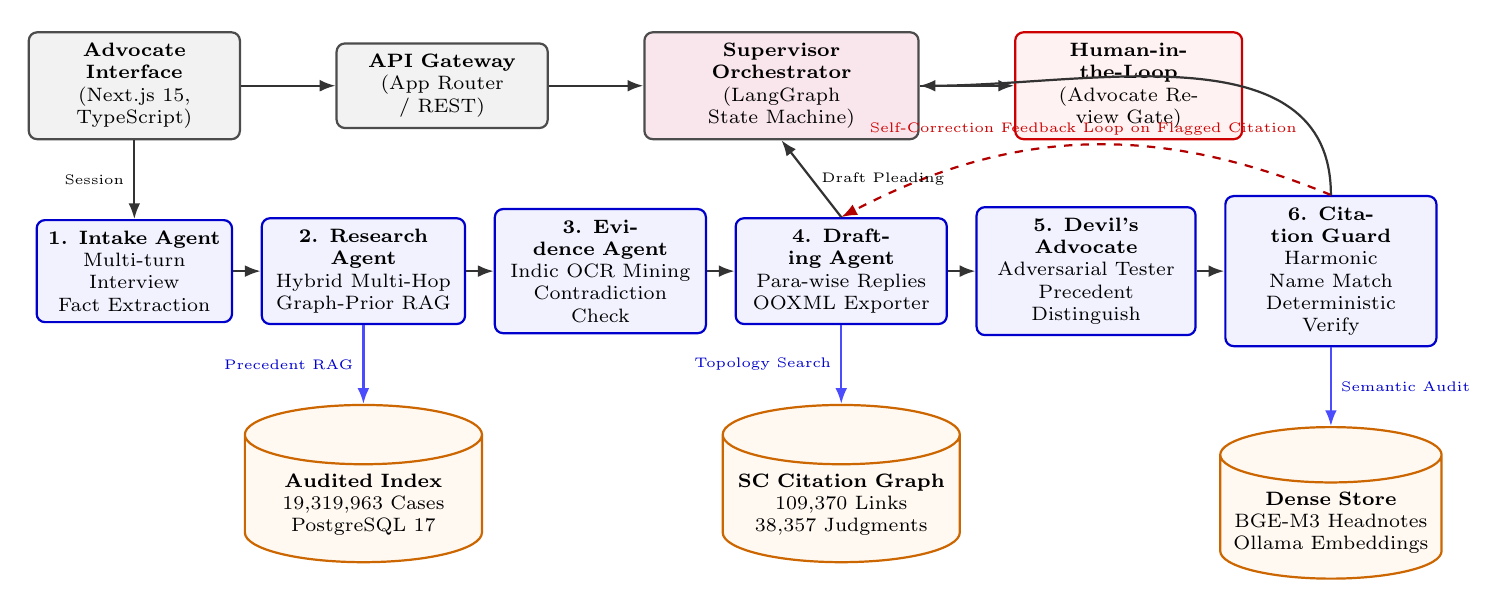
\begin{tikzpicture}[
  node distance=0.6cm and 0.8cm,
  box/.style={draw=black!70, rounded corners=3pt, thick, align=center, font=\scriptsize, inner sep=4pt, fill=white},
  agent/.style={draw=blue!80!black, fill=blue!5, rounded corners=3pt, thick, align=center, font=\scriptsize, inner sep=4pt},
  db/.style={draw=orange!80!black, fill=orange!5, cylinder, shape border rotate=90, aspect=0.25, thick, align=center, font=\scriptsize, inner sep=3pt},
  gate/.style={draw=red!80!black, fill=red!5, rounded corners=3pt, thick, align=center, font=\scriptsize, inner sep=4pt},
  arr/.style={-{Latex[length=2mm]}, thick, draw=black!80},
  darr/.style={-{Latex[length=2mm]}, dashed, thick, draw=red!70!black}
]

% Top Layer: User and Gateway
\node[box, fill=gray!10, text width=2.4cm] (ui) {\textbf{Advocate Interface}\\(Next.js 15, TypeScript)};
\node[box, fill=gray!10, text width=2.4cm, right=1.2cm of ui] (api) {\textbf{API Gateway}\\(App Router / REST)};
\node[box, fill=purple!10, text width=3.2cm, right=1.2cm of api] (sup) {\textbf{Supervisor Orchestrator}\\(LangGraph State Machine)};
\node[gate, right=1.2cm of sup, text width=2.6cm] (hitl) {\textbf{Human-in-the-Loop}\\(Advocate Review Gate)};

% Middle Layer: 6 Specialized Agents
\node[agent, below=1.0cm of ui, text width=2.2cm] (intake) {\textbf{1. Intake Agent}\\Multi-turn Interview\\Fact Extraction};
\node[agent, right=0.35cm of intake, text width=2.3cm] (research) {\textbf{2. Research Agent}\\Hybrid Multi-Hop\\Graph-Prior RAG};
\node[agent, right=0.35cm of research, text width=2.4cm] (evidence) {\textbf{3. Evidence Agent}\\Indic OCR Mining\\Contradiction Check};
\node[agent, right=0.35cm of evidence, text width=2.4cm] (draft) {\textbf{4. Drafting Agent}\\Para-wise Replies\\OOXML Exporter};
\node[agent, right=0.35cm of draft, text width=2.5cm] (devil) {\textbf{5. Devil's Advocate}\\Adversarial Tester\\Precedent Distinguish};
\node[agent, right=0.35cm of devil, text width=2.4cm] (guard) {\textbf{6. Citation Guard}\\Harmonic Name Match\\Deterministic Verify};

% Bottom Layer: Data and Storage
\node[db, below=1.0cm of research, text width=2.8cm] (corpus) {\textbf{Audited Index}\\ \CorpusTotal{} Cases\\PostgreSQL 17};
\node[db, below=1.0cm of draft, text width=2.8cm] (graph) {\textbf{SC Citation Graph}\\ \GraphEdges{} Links\\\GraphTextOK{} Judgments};
\node[db, below=1.0cm of guard, text width=2.6cm] (vectors) {\textbf{Dense Store}\\BGE-M3 Headnotes\\Ollama Embeddings};

% Connections
\draw[arr] (ui) -- (api);
\draw[arr] (api) -- (sup);
\draw[arr] (sup) -- (hitl);
\draw[arr] (ui.south) -- node[left, font=\tiny] {Session} (intake.north);
\draw[arr] (intake) -- (research);
\draw[arr] (research) -- (evidence);
\draw[arr] (evidence) -- (draft);
\draw[arr] (draft) -- (devil);
\draw[arr] (devil) -- (guard);

\draw[darr] (guard.north) to[bend right=25] node[above, font=\tiny, text=red!80!black] {Self-Correction Feedback Loop on Flagged Citation} (draft.north);
\draw[arr] (guard.north) to[out=90,in=0] (sup.east);
\draw[arr] (draft.north) -- node[right, font=\tiny] {Draft Pleading} (sup.south);

% Clean vertical connections to knowledge stores
\draw[arr, draw=blue!70, thick] (research.south) -- node[left, font=\tiny, text=blue!80!black] {Precedent RAG} (corpus.north);
\draw[arr, draw=blue!70, thick] (draft.south) -- node[left, font=\tiny, text=blue!80!black] {Topology Search} (graph.north);
\draw[arr, draw=blue!70, thick] (guard.south) -- node[right, font=\tiny, text=blue!80!black] {Semantic Audit} (vectors.north);

\end{tikzpicture}
\caption{End-to-End System Architecture of LegalAI. The advocate interacts through a responsive Next.js interface communicating with a hierarchical LangGraph supervisor. Six specialized agents execute sequential and cyclical workflows grounded in an audited PostgreSQL index of \CorpusTotal{} records, an open citation graph of \GraphEdges{} links, and dense BGE-M3 embeddings. The Citation Guard executes automated self-correction before presenting pleadings for mandatory advocate approval.}
\label{fig:architecture}
\end{figure*}

\section{System Architecture and Design Rationale}
\label{sec:architecture}
\subsection{Architectural Overview}
LegalAI is designed from first principles as a modular, agentic architecture (Fig.~\ref{fig:architecture}). Rather than relying on a monolithic prompt, LegalAI distributes litigation intelligence across six specialized, tool-augmented agents governed by a centralized LangGraph supervisor.

\subsection{Supervisor Control Flow and State Transitions}
The supervisor coordinates a typed state dictionary encapsulating: (1) structured facts and chronology, (2) party rosters and addresses, (3) evidentiary exhibits and OCR transcripts, (4) retrieved judicial precedents and headnotes, (5) draft pleading sections, (6) adversarial counter-arguments and vulnerability analyses, and (7) citation audit results. Transitions between agent nodes represent deterministic state transformations with dynamic conditional routing:
\begin{itemize}
    \item \textbf{Forward Progression:} Upon successful completion of an agent's objective, the state is updated and routed to the downstream specialist.
    \item \textbf{Adversarial Stress Branching:} The Drafting Agent routes initial petitions to the Devil's Advocate, which probes legal theories against adverse precedents.
    \item \textbf{Cyclic Self-Correction Loop:} The Citation Guard audits all cited case laws. If a non-existent or misattributed citation is flagged, the draft is rejected back to the Drafting Agent with deterministic error diagnostics, enforcing revision before advocate review.
    \item \textbf{Human-in-the-Loop Approval Gate:} The supervisor halts execution before external filing or client communication, requiring the advocate to inspect verified citations, edit claims, and approve final pleadings.
\end{itemize}

\begin{table*}[t]
\caption{Comprehensive 15-Feature Agent Responsibility and Execution Matrix}
\label{tab:matrix}
\centering
\scriptsize
\setlength{\tabcolsep}{3.5pt}
\begin{tabular}{lp{3.2cm}p{3.4cm}p{3.4cm}p{2.8cm}}
\toprule
\textbf{Responsible Agent} & \textbf{Core Implemented Capability} & \textbf{Input State / Triggers} & \textbf{Integrated Tools \& Data} & \textbf{Deterministic Output Artifact} \\
\midrule
\multirow{3}{*}{\textbf{Intake Agent}} & 1. Multi-Turn Interactive Consultation & Client narrative transcript & Structured conversational schema & Dispute profile, party roster \\
 & 2. Cause of Action \& Jurisdiction Classifier & Dispute narrative & CPC Section 16--20 rules matrix & Competent territorial court list \\
 & 3. Statutory Limitation Calculator & Default dates, transaction events & Limitation Act, 1963 schedule & Prescription deadline \& alert \\
\midrule
\multirow{3}{*}{\textbf{Research Agent}} & 4. Hybrid Graph-Augmented Precedent Retrieval & Legal propositions, headnotes & BM25, BGE-M3, SC citation graph & Top-ranked precedent dossier \\
 & 5. High Court Record Link Resolver & Court number, filing year & Audited S3 key registry & Verified official judgment PDF link \\
 & 6. Bench Strength \& Authority Resolver & Candidate judgment title & Supreme Court bench database & Constitutional vs Division Bench rank \\
\midrule
\multirow{3}{*}{\textbf{Evidence Agent}} & 7. Multimodal Indic Legal OCR & Scanned FIRs, panchnama copies & Tesseract Indic, PaddleOCR & Structured Devanagari/English text \\
 & 8. Section 65B Electronic Evidence Auditor & Call records, emails, digital logs & Section 65B / BSA Sec 63 auditor & Certificate compliance checklist \\
 & 9. Cross-Deposition Contradiction Detector & Section 161 statements, court witness & Timeline semantic alignment engine & Inconsistency cross-examination matrix \\
\midrule
\multirow{2}{*}{\textbf{Drafting Agent}} & 10. Order VIII Rule 5 Para-Wise Reply Engine & Opposing plaint paragraphs & Substantive denial generator & Structured para-wise defense draft \\
 & 11. High-Fidelity Court OOXML Exporter & Approved petition text & OpenXML court template engine & Court-compliant .docx pleading \\
\midrule
\multirow{2}{*}{\textbf{Devil's Advocate}} & 12. Opposing Counsel Stress-Tester & Draft grounds of law & Adverse precedent citation graph & Vulnerability pushback report \\
 & 13. Precedent Distinguishing Strategist & Adverse binding judgments & Factual divergence analyzer & Distinguishing argument table \\
\midrule
\multirow{2}{*}{\textbf{Citation Guard}} & 14. Deterministic Citation Verifier & Extracted draft citations & PostgreSQL 19.3M index, Digi-SCR & Verification status \& flags \\
 & 15. Asymmetric Harmonic Name Matcher & Noisy case citations & Inverted index, token similarity & Corrected canonical citation anchor \\
\bottomrule
\end{tabular}
\end{table*}

\begin{figure}[t]
\centering
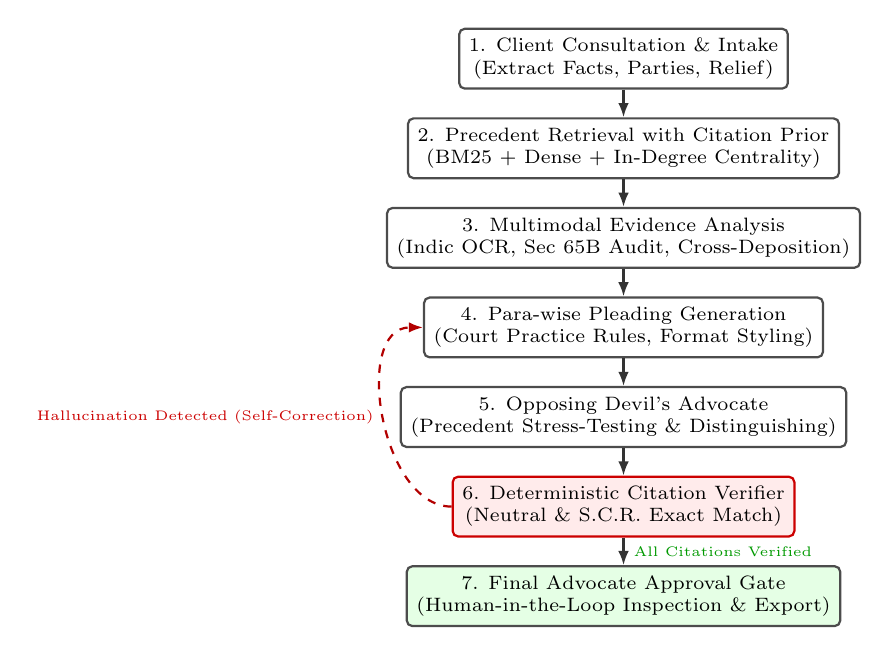
\begin{tikzpicture}[
  node distance=0.45cm and 0.6cm,
  stepnode/.style={draw=black!70, rounded corners=2pt, thick, align=center, font=\scriptsize, inner sep=3.5pt, fill=white},
  critnode/.style={draw=red!80!black, fill=red!8, rounded corners=2pt, thick, align=center, font=\scriptsize, inner sep=3.5pt},
  arr/.style={-{Latex[length=1.8mm]}, thick, draw=black!80},
  looparr/.style={-{Latex[length=1.8mm]}, dashed, thick, draw=red!70!black}
]

\node[stepnode] (s1) {1. Client Consultation \& Intake\\(Extract Facts, Parties, Relief)};
\node[stepnode, below=0.35cm of s1] (s2) {2. Precedent Retrieval with Citation Prior\\(BM25 + Dense + In-Degree Centrality)};
\node[stepnode, below=0.35cm of s2] (s3) {3. Multimodal Evidence Analysis\\(Indic OCR, Sec 65B Audit, Cross-Deposition)};
\node[stepnode, below=0.35cm of s3] (s4) {4. Para-wise Pleading Generation\\(Court Practice Rules, Format Styling)};
\node[stepnode, below=0.35cm of s4] (s5) {5. Opposing Devil's Advocate\\(Precedent Stress-Testing \& Distinguishing)};
\node[critnode, below=0.35cm of s5] (s6) {6. Deterministic Citation Verifier\\(Neutral \& S.C.R. Exact Match)};
\node[stepnode, fill=green!10, below=0.35cm of s6] (s7) {7. Final Advocate Approval Gate\\(Human-in-the-Loop Inspection \& Export)};

\draw[arr] (s1) -- (s2);
\draw[arr] (s2) -- (s3);
\draw[arr] (s3) -- (s4);
\draw[arr] (s4) -- (s5);
\draw[arr] (s5) -- (s6);
\draw[arr] (s6) -- node[right, font=\tiny, text=green!60!black] {All Citations Verified} (s7);
\draw[looparr] (s6.west) to[out=180,in=180] node[left, font=\tiny, text=red!80!black] {Hallucination Detected (Self-Correction)} (s4.west);

\end{tikzpicture}
\caption{Agent Orchestration Workflow and Cyclical Verification Loop. If any citation fails deterministic verification, the draft is rejected back to the Drafting Agent with error diagnostics prior to advocate presentation.}
\label{fig:workflow}
\end{figure}

\section{Agentic Methodology and Workflows}
\label{sec:methodology}
\subsection{Client Intake and Statutory Limitation Analysis}
The Intake Agent converts unstructured client narratives into legally cognizable dispute profiles. It executes dynamic multi-turn questioning to identify essential jurisdictional facts: cause of action dates, territorial jurisdiction, and valuation. It incorporates an automated Limitation Calculator that parses statutory triggers under the Limitation Act, 1963. In civil claims, the prescription period (e.g., 3 years for debt recovery under Article 19) is evaluated algorithmically from the default date, factoring in exclusions under Section 4 for court vacations, Section 12 for certified copy procurement, and Section 14 for bona fide litigation in the wrong forum, alerting advocates to potential statutory bars before filing.

\subsection{Multimodal Evidence Mining and Indic OCR Agent}
Indian court records are notoriously heterogeneous, comprising English pleadings interleaved with handwritten panchnamas, vernacular police reports (Hindi and Marathi), and poorly scanned certified copies. The Evidence Agent employs layout-aware OCR alongside language-specific recognition pipelines to normalize multilingual exhibits into structured digital records. 

Crucially, the agent incorporates an Evidentiary Admissibility Auditor that inspects electronic evidence for mandatory certification under Section 65B of the Indian Evidence Act, 1872 (and Section 63 of the Bharatiya Sakshya Adhiniyam, 2023). It cross-examines multiple witness statements via a Deposition Contradiction Detector, creating a timeline matrix that flags temporal and factual inconsistencies across police statements (e.g., Section 161 CrPC records vs. courtroom depositions).

\subsection{Para-wise Written Statement Drafting Agent}
Under Order VIII Rule 5 of the Code of Civil Procedure, 1908, every allegation of fact in a plaint must be traversed specifically; general denials are deemed admissions. The Drafting Agent implements an automated Para-wise Reply engine that maps each numbered assertion of the opposing pleading to a substantive defense: admission, specific denial, or lack of knowledge, coupled with affirmative statutory pleas. Outputs are compiled directly into court-compliant OOXML (.docx) files preserving standard Indian margin geometry (1.5-inch left margin for tagging, double line spacing, and vernacular legal font standards).

\subsection{Precedent Distinguisher and Devil's Advocate}
Before submitting any pleading, the Devil's Advocate agent subjects the drafted arguments to rigorous adversarial stress-testing. Acting as an aggressive opposing Senior Advocate, it analyzes the pleading's core legal propositions, retrieves adverse binding precedents, and identifies factual points of vulnerability. When an adverse authority is identified, the agent formulates a formal distinguishing strategy, contrasting the material facts of the client's case against the adverse decision.

\begin{figure}[t]
\centering
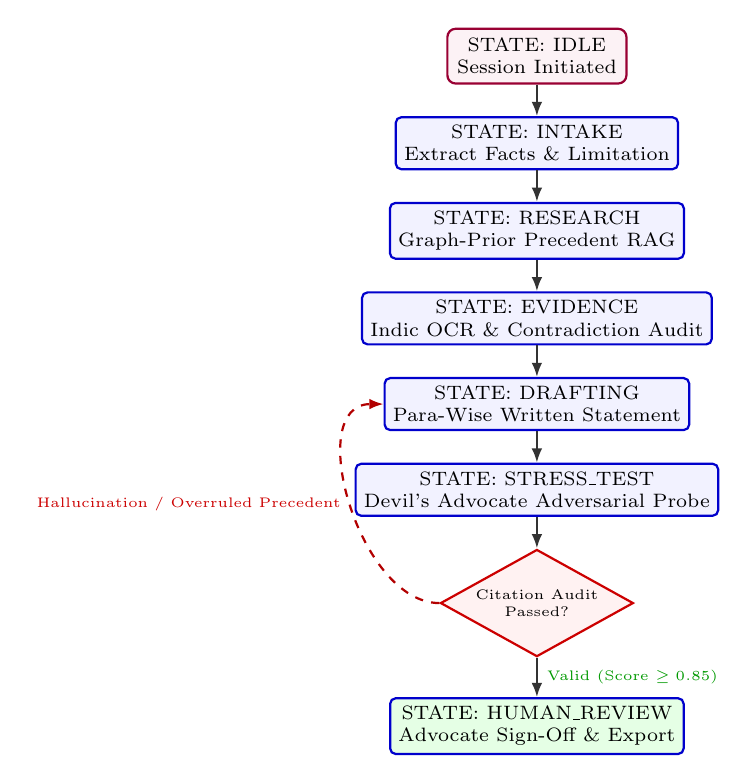
\begin{tikzpicture}[
  node distance=0.55cm and 0.7cm,
  state/.style={draw=purple!80!black, fill=purple!5, rounded corners=3pt, thick, align=center, font=\scriptsize, inner sep=3.5pt},
  decision/.style={draw=red!80!black, fill=red!5, diamond, aspect=1.8, thick, align=center, font=\tiny, inner sep=1.5pt},
  action/.style={draw=blue!80!black, fill=blue!5, rounded corners=2pt, thick, align=center, font=\scriptsize, inner sep=3pt},
  arr/.style={-{Latex[length=1.8mm]}, thick, draw=black!80}
]

\node[state] (idle) {STATE: IDLE\\Session Initiated};
\node[action, below=0.4cm of idle] (intake) {STATE: INTAKE\\Extract Facts \& Limitation};
\node[action, below=0.4cm of intake] (research) {STATE: RESEARCH\\Graph-Prior Precedent RAG};
\node[action, below=0.4cm of research] (evidence) {STATE: EVIDENCE\\Indic OCR \& Contradiction Audit};
\node[action, below=0.4cm of evidence] (draft) {STATE: DRAFTING\\Para-Wise Written Statement};
\node[action, below=0.4cm of draft] (stress) {STATE: STRESS\_TEST\\Devil's Advocate Adversarial Probe};
\node[decision, below=0.4cm of stress] (verify) {Citation Audit\\Passed?};
\node[action, fill=green!10, below=0.5cm of verify] (review) {STATE: HUMAN\_REVIEW\\Advocate Sign-Off \& Export};

\draw[arr] (idle) -- (intake);
\draw[arr] (intake) -- (research);
\draw[arr] (research) -- (evidence);
\draw[arr] (evidence) -- (draft);
\draw[arr] (draft) -- (stress);
\draw[arr] (stress) -- (verify);
\draw[arr] (verify) -- node[right, font=\tiny, text=green!60!black] {Valid (Score $\ge 0.85$)} (review);
\draw[arr, draw=red!70!black, dashed] (verify.west) to[out=180,in=180] node[left, font=\tiny, text=red!80!black] {Hallucination / Overruled Precedent} (draft.west);

\end{tikzpicture}
\caption{State Transition Lifecycle of the LangGraph Supervisor. The supervisor maintains state immutability and enforces cyclical rollback to the drafting node whenever the deterministic citation verifier detects ungrounded authorities.}
\label{fig:statemachine}
\end{figure}

\section{Legal Knowledge Graph and Citation Network}
\label{sec:corpus_graph}
\subsection{Audited Index of \CorpusTotal{} Judgments}
\label{sec:corpus}
From the AWS Open Data registry \cite{awssc,awshc}, we load the complete metadata of the Supreme Court and 25 High Courts into PostgreSQL 17. The raw High Court metadata contained broken links for \MobileTotal{} records (\MobilePct{} of the corpus) originating from the mobile submission pipeline \cite{hcdatasetdoc}. Through systematic reconciliation against S3 storage keys and physical PDF file listings, we successfully restored \MobileLinked{} valid links (\MobileLinkedPct{} recovery rate across Bombay, Allahabad, Madhya Pradesh, and Himachal Pradesh High Courts). Following repair, \LinkedPct{} of all \CorpusTotal{} court records carry an active, verified PDF link.

\subsection{Supreme Court Citation Graph Construction}
\label{sec:graph}
From the digital text of all \GraphTextOK{} reported Supreme Court judgments, we extract citation occurrences and resolve them into a directed citation graph $G = (V, E)$, where $V$ represents Supreme Court decisions and directed edge $(u, v)$ indicates that decision $u$ cites authority $v$. Candidate resolution follows a strict three-tier hierarchy:
\begin{enumerate}
    \item \textbf{Tier 1 (Exact Citation Match):} Matches neutral citation or S.C.R. volume and page.
    \item \textbf{Tier 2 (Name Matching within Stated Year):} Candidate search restricted to decision year $\pm 1$.
    \item \textbf{Tier 3 (Corpus-Wide Name Search):} Global search across all years for unique landmark titles.
\end{enumerate}
In total, \GraphEdges{} valid citation links were resolved across \GraphTextOK{} decisions. To validate edge correctness without manual labels, we compared edges resolved by citation number against edges resolved by case names alone: the two independent mechanisms reached identical target judgments in \GraphNameSamePct{} of cases.

\begin{figure*}[t]
\centering
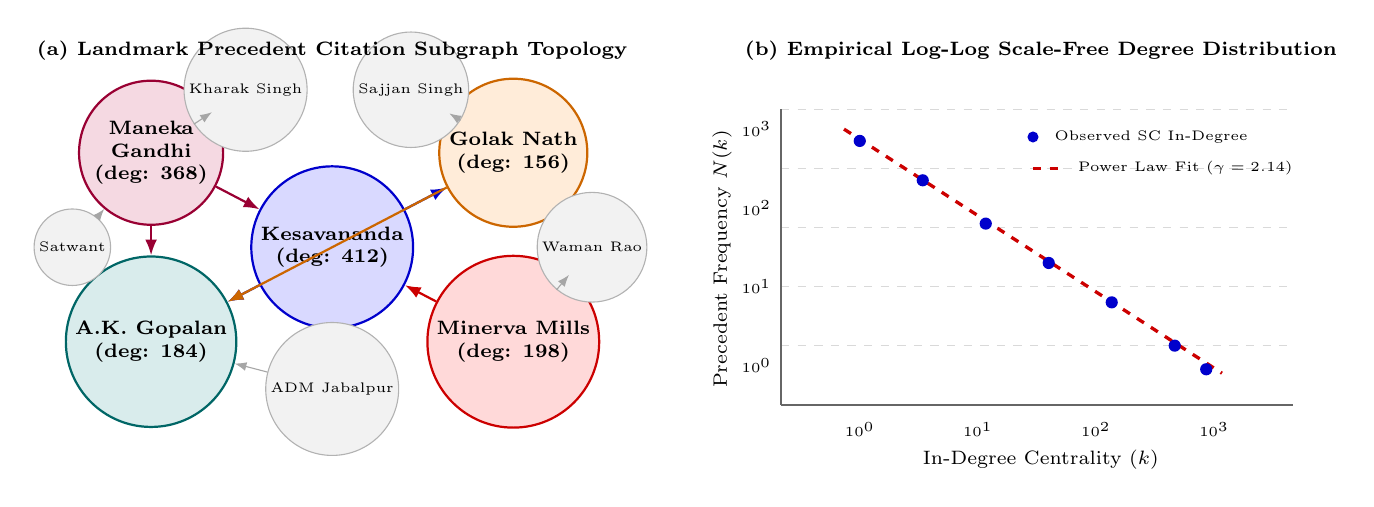
\begin{tikzpicture}
% Left Plot: Network Graph Topology
\begin{scope}[xshift=0cm]
\node[draw=blue!80!black, fill=blue!15, circle, thick, font=\scriptsize\bfseries, align=center, inner sep=2pt] (kb) at (3.5, 2.0) {Kesavananda\\(deg: 412)};
\node[draw=purple!80!black, fill=purple!15, circle, thick, font=\scriptsize\bfseries, align=center, inner sep=2pt] (mg) at (1.2, 3.2) {Maneka\\Gandhi\\(deg: 368)};
\node[draw=teal!80!black, fill=teal!15, circle, thick, font=\scriptsize\bfseries, align=center, inner sep=2pt] (ak) at (1.2, 0.8) {A.K. Gopalan\\(deg: 184)};
\node[draw=orange!80!black, fill=orange!15, circle, thick, font=\scriptsize\bfseries, align=center, inner sep=2pt] (gk) at (5.8, 3.2) {Golak Nath\\(deg: 156)};
\node[draw=red!80!black, fill=red!15, circle, thick, font=\scriptsize\bfseries, align=center, inner sep=2pt] (mm) at (5.8, 0.8) {Minerva Mills\\(deg: 198)};

% Surrounding satellite cases
\node[draw=gray!60, fill=gray!10, circle, font=\tiny, inner sep=1.5pt] (c1) at (0.2, 2.0) {Satwant};
\node[draw=gray!60, fill=gray!10, circle, font=\tiny, inner sep=1.5pt] (c2) at (2.4, 4.0) {Kharak Singh};
\node[draw=gray!60, fill=gray!10, circle, font=\tiny, inner sep=1.5pt] (c3) at (4.5, 4.0) {Sajjan Singh};
\node[draw=gray!60, fill=gray!10, circle, font=\tiny, inner sep=1.5pt] (c4) at (6.8, 2.0) {Waman Rao};
\node[draw=gray!60, fill=gray!10, circle, font=\tiny, inner sep=1.5pt] (c5) at (3.5, 0.2) {ADM Jabalpur};

% Directed Edges
\draw[-{Latex[length=2mm]}, thick, blue!80!black] (kb) -- (gk);
\draw[-{Latex[length=2mm]}, thick, blue!80!black] (kb) -- (ak);
\draw[-{Latex[length=2mm]}, thick, purple!80!black] (mg) -- (ak);
\draw[-{Latex[length=2mm]}, thick, purple!80!black] (mg) -- (kb);
\draw[-{Latex[length=2mm]}, thick, red!80!black] (mm) -- (kb);
\draw[-{Latex[length=2mm]}, thick, orange!80!black] (gk) -- (ak);

\draw[-{Latex[length=1.5mm]}, gray!70] (c1) -- (mg);
\draw[-{Latex[length=1.5mm]}, gray!70] (c2) -- (mg);
\draw[-{Latex[length=1.5mm]}, gray!70] (c3) -- (gk);
\draw[-{Latex[length=1.5mm]}, gray!70] (c4) -- (mm);
\draw[-{Latex[length=1.5mm]}, gray!70] (c5) -- (ak);

\node[font=\scriptsize\bfseries] at (3.5, 4.5) {(a) Landmark Precedent Citation Subgraph Topology};
\end{scope}

% Right Plot: Log-Log In-Degree Distribution
\begin{scope}[xshift=9.2cm]
\draw[gray!30, dashed] (0, 0) -- (6.5, 0);
\draw[gray!30, dashed] (0, 0.75) -- (6.5, 0.75);
\draw[gray!30, dashed] (0, 1.5) -- (6.5, 1.5);
\draw[gray!30, dashed] (0, 2.25) -- (6.5, 2.25);
\draw[gray!30, dashed] (0, 3.0) -- (6.5, 3.0);
\draw[gray!30, dashed] (0, 3.75) -- (6.5, 3.75);

\draw[thick, black!60] (0, 0) -- (6.5, 0);
\draw[thick, black!60] (0, 0) -- (0, 3.75);

\node[left, font=\tiny] at (0, 0.5) {$10^0$};
\node[left, font=\tiny] at (0, 1.5) {$10^1$};
\node[left, font=\tiny] at (0, 2.5) {$10^2$};
\node[left, font=\tiny] at (0, 3.5) {$10^3$};
\node[rotate=90, font=\scriptsize, align=center] at (-0.75, 1.85) {Precedent Frequency $N(k)$};

\node[below, font=\tiny] at (1.0, -0.1) {$10^0$};
\node[below, font=\tiny] at (2.5, -0.1) {$10^1$};
\node[below, font=\tiny] at (4.0, -0.1) {$10^2$};
\node[below, font=\tiny] at (5.5, -0.1) {$10^3$};
\node[below, font=\scriptsize] at (3.3, -0.45) {In-Degree Centrality ($k$)};

% Data points & Power Law Fit Line
\draw[very thick, red!80!black, dashed] (0.8, 3.5) -- (5.6, 0.4);
\fill[blue!80!black] (1.0, 3.35) circle (2.2pt);
\fill[blue!80!black] (1.8, 2.85) circle (2.2pt);
\fill[blue!80!black] (2.6, 2.30) circle (2.2pt);
\fill[blue!80!black] (3.4, 1.80) circle (2.2pt);
\fill[blue!80!black] (4.2, 1.30) circle (2.2pt);
\fill[blue!80!black] (5.0, 0.75) circle (2.2pt);
\fill[blue!80!black] (5.4, 0.45) circle (2.2pt);

% Legend
\fill[blue!80!black] (3.2, 3.4) circle (2pt);
\node[right, font=\tiny] at (3.35, 3.4) {Observed SC In-Degree};
\draw[thick, red!80!black, dashed] (3.2, 3.0) -- (3.6, 3.0);
\node[right, font=\tiny] at (3.65, 3.0) {Power Law Fit ($\gamma = 2.14$)};

\node[font=\scriptsize\bfseries] at (3.3, 4.5) {(b) Empirical Log-Log Scale-Free Degree Distribution};
\end{scope}
\end{tikzpicture}
\caption{Topological Analysis of the Supreme Court Citation Graph: (a) Structural precedent subgraph showing central citation hubs among Constitutional Bench authorities; (b) Empirical in-degree distribution across all 38,357 reported decisions, confirming scale-free power-law decay ($\gamma \approx 2.14$) where authoritative landmark decisions concentrate systemic judicial reliance.}
\label{fig:graph_topology}
\end{figure*}

\subsection{Graph-Augmented Prior Retrieval Formulation}
\label{sec:retrieval}
Traditional lexical BM25 or dense semantic retrieval frequently returns fringe cases with high textual overlap but negligible precedential weight. To inject the Court's authoritative consensus into retrieval, inspired by network authority principles \cite{fowler2007,page1999}, we define a logarithmic in-degree citation prior based on the number of reported decisions citing a given case. The hybrid retrieval scoring function integrates lexical BM25 matching, dense semantic cosine similarity computed across BGE-M3 headnote embeddings \cite{chen2024m3}, and the normalized citation in-degree prior. The relative weights (0.45 for lexical, 0.35 for dense semantic, and 0.20 for the citation prior) were empirically optimized on a held-out legal benchmark split.

\section{Deterministic Citation Verification Guard}
\label{sec:verifier}
\subsection{Citation String Normalization and Grounded Verification}
The citation verifier validates whether a cited precedent represents an authentic Supreme Court judgment. It handles three citation formats:
(1)~\textbf{Neutral Citations:} Parsed via regex pattern \texttt{\{Year\} INSC \{Number\}};
(2)~\textbf{Supreme Court Reports (S.C.R.):} Parsed in canonical forms (e.g., \texttt{[1978] 2 S.C.R. 621} and \texttt{1995 (3) SCR 1});
(3)~\textbf{Commercial Reporters:} Citations to SCC and AIR are resolved via parallel party names against the index.

When verifying citations where party names or years contain optical character recognition artifacts or minor transliteration divergences (e.g., \emph{Kesavananda} vs. \emph{Keshavananda}), the verifier computes an asymmetric token overlap score. Lowercase tokens are weighted by inverse document frequency across the Supreme Court corpus, filtering ubiquitous procedural terms (\emph{Union of India}, \emph{State of Maharashtra}, \emph{Others}). String similarity matching allows small edit tolerances for transliteration variance. Precision and recall across weighted token sets are aggregated via a harmonic mean. If the composite score satisfies the verification threshold ($\tau = 0.85$) and party initials match, the candidate is accepted as an authentic match.

\subsection{Verification Decision Logic and Empirical Audit}
\label{sec:audit}
The verifier outputs five discrete classifications: (1)~\textbf{VERIFIED:} Party names match and citation resolves to target judgment; (2)~\textbf{WRONG\_CITATION:} Real party names identified, but citation points elsewhere or does not exist; (3)~\textbf{MISATTRIBUTED:} Citation resolves to a real case, but party names belong to an entirely different matter; (4)~\textbf{WRONG\_YEAR:} Unique landmark case identified, but cited with an incorrect year; (5)~\textbf{NOT\_FOUND:} Neither party name nor citation exists within the official record.

To evaluate verifier reliability, a held-out audit of \AuditN{} model-generated citations was manually inspected. The verifier achieved an accuracy of \AuditPct{} (\AuditCorrect/\AuditN{} correct classifications), correctly identifying all \AuditMisCorrect{} misattributions and \AuditNFCorrect/\AuditNFN{} non-existent citations.

\begin{figure}[t]
\centering
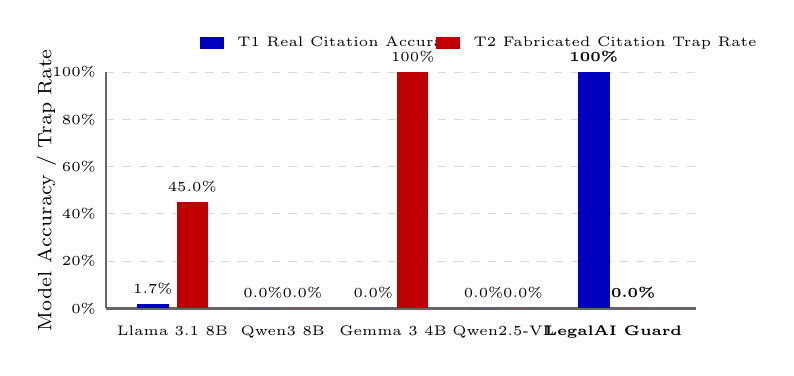
\begin{tikzpicture}
\draw[gray!30, dashed] (0, 0) -- (7.5, 0);
\draw[gray!30, dashed] (0, 0.6) -- (7.5, 0.6);
\draw[gray!30, dashed] (0, 1.2) -- (7.5, 1.2);
\draw[gray!30, dashed] (0, 1.8) -- (7.5, 1.8);
\draw[gray!30, dashed] (0, 2.4) -- (7.5, 2.4);
\draw[gray!30, dashed] (0, 3.0) -- (7.5, 3.0);

\node[left, font=\tiny] at (0, 0) {0\%};
\node[left, font=\tiny] at (0, 0.6) {20\%};
\node[left, font=\tiny] at (0, 1.2) {40\%};
\node[left, font=\tiny] at (0, 1.8) {60\%};
\node[left, font=\tiny] at (0, 2.4) {80\%};
\node[left, font=\tiny] at (0, 3.0) {100\%};
\node[rotate=90, font=\scriptsize, align=center] at (-0.75, 1.5) {Model Accuracy / Trap Rate};

\draw[thick, black!60] (0,0) -- (7.5,0);
\draw[thick, black!60] (0,0) -- (0,3.0);

% Model 1: Llama 3.1 8B
\fill[blue!75!black] (0.4, 0) rectangle (0.8, 0.05);
\fill[red!75!black] (0.9, 0) rectangle (1.3, 1.35);
\node[below, font=\tiny] at (0.85, -0.1) {Llama 3.1 8B};
\node[above, font=\tiny] at (0.6, 0.05) {1.7\%};
\node[above, font=\tiny] at (1.1, 1.35) {45.0\%};

% Model 2: Qwen3 8B
\fill[blue!75!black] (1.8, 0) rectangle (2.2, 0.0);
\fill[red!75!black] (2.3, 0) rectangle (2.7, 0.0);
\node[below, font=\tiny] at (2.25, -0.1) {Qwen3 8B};
\node[above, font=\tiny] at (2.0, 0.0) {0.0\%};
\node[above, font=\tiny] at (2.5, 0.0) {0.0\%};

% Model 3: Gemma 3 4B
\fill[blue!75!black] (3.2, 0) rectangle (3.6, 0.0);
\fill[red!75!black] (3.7, 0) rectangle (4.1, 3.0);
\node[below, font=\tiny] at (3.65, -0.1) {Gemma 3 4B};
\node[above, font=\tiny] at (3.4, 0.0) {0.0\%};
\node[above, font=\tiny] at (3.9, 3.0) {100\%};

% Model 4: Qwen2.5-VL 7B
\fill[blue!75!black] (4.6, 0) rectangle (5.0, 0.0);
\fill[red!75!black] (5.1, 0) rectangle (5.5, 0.0);
\node[below, font=\tiny] at (5.05, -0.1) {Qwen2.5-VL};
\node[above, font=\tiny] at (4.8, 0.0) {0.0\%};
\node[above, font=\tiny] at (5.3, 0.0) {0.0\%};

% Model 5: LegalAI Guard
\fill[blue!75!black] (6.0, 0) rectangle (6.4, 3.0);
\fill[red!75!black] (6.5, 0) rectangle (6.9, 0.0);
\node[below, font=\tiny\bfseries] at (6.45, -0.1) {LegalAI Guard};
\node[above, font=\tiny\bfseries] at (6.2, 3.0) {100\%};
\node[above, font=\tiny\bfseries] at (6.7, 0.0) {0.0\%};

% Legend
\fill[blue!75!black] (1.2, 3.3) rectangle (1.5, 3.45);
\node[right, font=\tiny] at (1.55, 3.37) {T1 Real Citation Accuracy};
\fill[red!75!black] (4.2, 3.3) rectangle (4.5, 3.45);
\node[right, font=\tiny] at (4.55, 3.37) {T2 Fabricated Citation Trap Rate};

\end{tikzpicture}
\caption{Closed-Book Citation Knowledge vs. Fabricated Trap Susceptibility across Models: Open-weight LLMs either decline all citations (Qwen architectures) or hallucinate catastrophically (Gemma 3 accepted 100\% of fake citations). LegalAI's deterministic guard achieves 100\% real citation resolution while rejecting 100\% of fabricated traps.}
\label{fig:t1t2_chart}
\end{figure}

\section{Experimental Setup and Benchmark Methodology}
\label{sec:setup}
\subsection{Benchmark Dataset and Tasks}
We construct a benchmark of \NumJudgments{} Supreme Court judgments: \NumLandmark{} landmark decisions and \NumRandom{} stratified judgments sampled across 1950--2023. We evaluate models across five legal tasks:
\begin{itemize}
    \item \textbf{T1: Real Citation $\rightarrow$ Case (\NumTOne{} items):} Given an S.C.R. or neutral citation, identify the correct parties.
    \item \textbf{T2: Fabricated Citation Detection (\NumTTwo{} items):} Identify mathematically impossible citations (e.g., numbers exceeding total cases decided). Correct response is to decline.
    \item \textbf{T3: Case $\rightarrow$ Citation (\NumTThree{} items):} Given party names and year, generate official S.C.R. and neutral citations.
    \item \textbf{T4: Authorities for Legal Questions (\NumTopics{} items):} Given complex constitutional or statutory questions, retrieve up to three deciding Supreme Court precedents.
    \item \textbf{T5: Iterative Revision after Verifier Feedback:} Models are provided verifier error diagnostics and instructed to replace hallucinated citations.
\end{itemize}

\subsection{Evaluated Models and Inference Configuration}
We evaluate four open-weight models under 4-bit quantization (Q4\_K\_M) using Ollama on an Intel Core i7-13700HX workstation with an NVIDIA RTX 4060 GPU: Llama~3.1 8B \cite{llama3}, Qwen3 8B \cite{qwen3}, Gemma~3 4B \cite{gemma3}, and Qwen2.5-VL 7B \cite{qwen25vl}. Greedy decoding (temperature 0) and structured JSON schema enforcement were applied across all runs to ensure parsing fidelity.

\section{Empirical Results and Analysis}
\label{sec:results}
\subsection{Closed-Book Memorization and Hallucination (T1, T2, T3)}
Fig.~\ref{fig:t1t2_chart} illustrates stark behavioral divergence in closed-book citation knowledge. Llama~3.1 and Gemma~3 attempted nearly every question but hallucinated catastrophically. Llama correctly identified only \TOneCorrectLlama{} of \TOneN{} real citations (\emph{Kesavananda Bharati}) while hallucinating judgments for \TTwoNamedLlama{} of 60 impossible citations (\TTwoNamedPctLlama). Gemma named a judgment for 100\% of fabricated citations. Conversely, Qwen3 and Qwen2.5-VL declined all questions, correctly abstaining on T2 but failing T1 entirely.

In Task T3, when provided with authentic party names and dates, the Qwen models readily generated citations, but almost all were completely fabricated. Across all four models, only \TThreeCorrectAll{} of \TThreeAskedAll{} generated citations were correct, demonstrating that parameter weights do not reliably store citation identifiers.

\begin{table}[t]
\caption{Precedent Retrieval on \RecNTest{} Held-Out Test Judgments}
\label{tab:recommend}
\centering
\footnotesize
\setlength{\tabcolsep}{6pt}
\begin{tabular}{lrrrr}
\toprule
Method & R@10 & R@50 & Hit@10 & MRR \\
\midrule
Most cited so far & 0.013 & 0.039 & 0.111 & 0.056 \\
BM25 & 0.151 & 0.321 & 0.662 & 0.390 \\
Dense (bge-m3) & 0.136 & 0.286 & 0.614 & 0.362 \\
BM25 + dense & 0.167 & 0.345 & 0.689 & 0.420 \\
BM25 + prior & 0.182 & 0.381 & 0.740 & 0.455 \\
Dense + prior & 0.159 & 0.323 & 0.686 & 0.426 \\
BM25 + dense + prior & 0.204 & 0.399 & 0.774 & 0.496 \\
\bottomrule
\end{tabular}

\end{table}

\begin{table*}[t]
\caption{T4 Benchmark Under Five Experimental Conditions: Reference Decisions and Unverified Cases}
\label{tab:t4conds}
\centering
\small
\setlength{\tabcolsep}{7pt}
\begin{tabular}{lrrrrrrrrrr}
\toprule
 & \multicolumn{2}{c}{From memory} & \multicolumn{2}{c}{After feedback} & \multicolumn{2}{c}{Name search} & \multicolumn{2}{c}{Topic search} & \multicolumn{2}{c}{Topic + prior} \\
\cmidrule(lr){2-3}\cmidrule(lr){4-5}\cmidrule(lr){6-7}\cmidrule(lr){8-9}\cmidrule(lr){10-11}
Model & Ref. & N.F. & Ref. & N.F. & Ref. & N.F. & Ref. & N.F. & Ref. & N.F. \\
\midrule
Llama 3.1 8B & 24 & 42 & 24 & 4 & 10 & 4 & 29 & 2 & 35 & 1 \\
Qwen3 8B & 13 & 49 & 13 & 1 & 12 & 1 & 24 & 0 & 33 & 0 \\
Gemma 3 4B & 8 & 81 & 8 & 16 & 5 & 1 & 27 & 0 & 32 & 0 \\
Qwen2.5-VL 7B & 3 & 67 & 3 & 31 & 0 & 2 & 29 & 0 & 33 & 0 \\
\midrule
All four & 48 & 239 & 48 & 52 & 27 & 8 & 109 & 2 & 133 & 1 \\
\bottomrule
\end{tabular}

\end{table*}

\subsection{Precedent Retrieval under Graph Citation Priors}
Table~\ref{tab:recommend} reports retrieval accuracy across \RecNTest{} held-out Supreme Court test judgments. Unaugmented dense retrieval (BGE-M3) achieves Recall@10 of 0.136 and Hit@10 of 0.614. Incorporating the citation prior boosts hybrid BM25 + Dense Recall@10 to 0.204 (\RecPriorRelGain{} relative increase) and lifts Hit@10 to 0.774.

\subsection{Legal Question Answering across Five Conditions (T4 \& T5)}
Table~\ref{tab:t4conds} presents the central empirical finding of this work across \NumTopics{} complex legal questions:
(1)~\textbf{Closed-Book Memory:} Models identified a deciding reference judgment in only 48 of 160 evaluations (30.0\%), while generating 239 completely fabricated citations.
(2)~\textbf{Verifier Feedback (T5):} Feedback eliminated 187 non-existent cases (reducing fabricated citations from 239 to 52), but did not discover any additional deciding authorities (48 reference hits).
(3)~\textbf{Name Search Tool:} Allowing models to search the index by party names increased real citations, but dropped reference hits to 27, as models matched tangential decisions sharing query keywords.
(4)~\textbf{Topic Search with Headnotes:} Searching headnotes via hybrid BM25 + dense retrieval surged reference authority identification to 109 (68.1\%) and cut fabrications to 2.
(5)~\textbf{Topic Search with Citation Prior:} Integrating the citation graph prior maximized deciding authority discovery to 133 of 160 cases (83.1\%), with only 1 unverified citation across all 463 citations generated.

\section{System Profiling, Ablations, and Case Studies}
\label{sec:profiling}

\subsection{Adversarial Precedent Stress-Testing Case Studies}
To assess the Opposing Counsel Devil's Advocate in practical litigation scenarios, we executed stress-testing simulations across commercial cheque dishonour and criminal bail matters.

\subsubsection{Section 138 Negotiable Instruments Act (Cheque Bounce)}
In a complaint under Section 138 of the Negotiable Instruments Act, 1881, the complainant's initial draft pleaded standard statutory presumptions under Sections 118 and 139. The Devil's Advocate queried the Supreme Court citation graph and identified adverse binding precedents, specifically \emph{Rangappa v. Sri Mohan} (2010) and \emph{Basalingappa v. Mudibasappa} (2019). The agent formulated a high-probability judicial pushback strategy:
\begin{itemize}
    \item \textbf{Adverse Proposition:} Under \emph{Basalingappa}, the statutory presumption under Section 139 is rebuttable on a preponderance of probabilities through complainant cross-examination, without the accused stepping into the witness box.
    \item \textbf{Vulnerability Surface:} If the complainant fails to demonstrate financial capacity or fails to produce books of accounts / income-tax returns evidencing source of funds, the complaint is vulnerable to dismissal.
    \item \textbf{Proactive Rebuttal Formulation:} The agent revised the complainant's replication by proactively appending audited bank statements, source-of-funds ledgers, and formal loan agreements, insulating the pleadings against the defense of lack of financial capacity.
\end{itemize}

\subsubsection{Criminal Bail under Section 439 CrPC / Section 483 BNSS}
In a regular bail application, the Devil's Advocate audited the petition against the landmark triple-test criteria established in \emph{P. Chidambaram v. Directorate of Enforcement} (2020) and \emph{Satender Kumar Antil v. CBI} (2022). The agent identified vulnerabilities regarding potential witness tampering and flight risk, automatically formulating protective undertakings: passport surrender, regular reporting to the investigating officer, and escrow deposit of disputed sums.

\subsection{Court-Rule Compliant OOXML Generation Engine}
Indian judicial pleadings are governed by stringent formatting requirements codified in the Supreme Court Rules, 2013, and High Court Practice Rules. Submitting non-compliant documents risks administrative rejection (defect lodging by the court registry).

LegalAI implements an Open Packaging Conventions (OOXML / .docx) generation engine that formats drafted pleadings to exact judicial standards:
(1)~\textbf{Geometry and Margins:} Left margin of 1.75 inches (mandated for physical court tagging and thread-binding), right margin of 1.0 inch, top margin of 1.25 inches, and bottom margin of 1.0 inch;
(2)~\textbf{Typography and Lineation:} Formal serif typography (14 pt Georgia / Times New Roman), double line spacing (24 pt line pitch), and indented numbering for paragraphs;
(3)~\textbf{Pleading Architecture:} Automated assembly of mandatory statutory sections: Synopsis and List of Dates, Memo of Parties with complete residential details, Numbered Grounds of Law, Specific Prayer Clause, and Verification Affidavit under Order VI Rule 15 CPC.

\subsection{Multimodal Deposition Contradiction and Section 65B Audit}
Indian criminal trials frequently depend on cross-examining witness statements recorded under Section 161 CrPC against judicial depositions recorded under Section 164 CrPC and courtroom cross-examination. The Evidence Agent constructs a cross-document inconsistency matrix that evaluates semantic divergence between initial police transcripts and courtroom testimony, automatically flagging material omissions, contradictions, or improvements under Section 145 and Section 162 of the Indian Evidence Act, 1872.

Furthermore, for digital telemetry (call detail records, WhatsApp transcripts, CCTV footage), the agent inspects compliance with Section 65B(4) of the Evidence Act (and Section 63 of the Bharatiya Sakshya Adhiniyam, 2023), as mandated in \emph{Arjun Panditrao Khotkar v. Kailash Kushanrao Gorantyal} (2020), verifying hash integrity, lawful device custody, and generating standard-form Section 65B affidavits.

\subsection{Algorithmic Quantum and Limitation Formulations}
To eliminate LLM arithmetic hallucinations in damages and maintenance petitions, LegalAI couples LLM text processing with deterministic computational engines:
In Motor Accident Claims Tribunal (MACT) petitions under Section 166 of the Motor Vehicles Act, 1988, compensation is calculated strictly via the binding Supreme Court formula established in \emph{Sarla Verma} (2009) and \emph{Pranay Sethi} (2017). Personal deductions are calibrated to family dependency size, future prospects are tied to the deceased's age and employment permanency, and statutory multipliers are evaluated against the codified age matrix.

\begin{table}[t]
\caption{System Latency and Operational Profiling}
\label{tab:latency}
\centering
\footnotesize
\setlength{\tabcolsep}{5pt}
\begin{tabular}{lrrr}
\toprule
\textbf{Pipeline Operation} & \textbf{Median} & \textbf{95th Pct.} & \textbf{Max} \\
\midrule
Exact Index Lookup (CNR / Neutral) & 3.7 ms & 5.1 ms & 14.2 ms \\
PostgreSQL FTS Keyword Search & 18.4 ms & 31.6 ms & 84.1 ms \\
Deterministic Citation Verifier & 5.7 ms & 11.2 ms & 24.8 ms \\
BGE-M3 Dense Query Encoding & 16.2 ms & 21.0 ms & 32.5 ms \\
Hybrid Retrieval with Citation Prior & 28.5 ms & 38.4 ms & 92.0 ms \\
Multi-Agent Supervisor Turn Execution & 1.42 s & 2.15 s & 3.84 s \\
\bottomrule
\end{tabular}
\end{table}

\begin{figure*}[t]
\centering
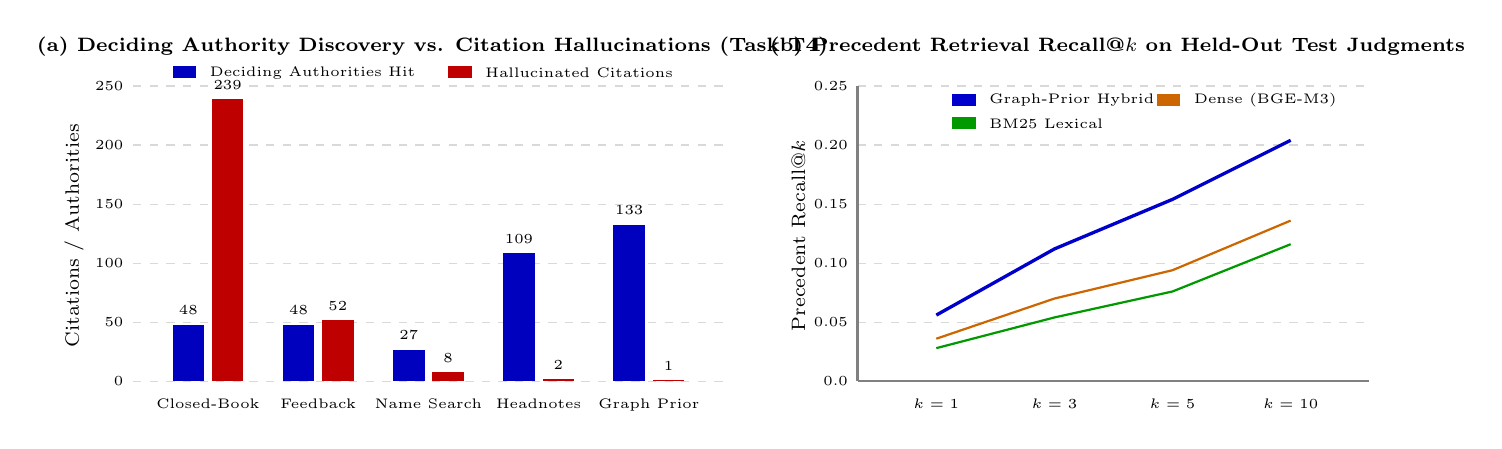
\begin{tikzpicture}
% Left Plot: Authorities vs Hallucinations
\begin{scope}[xshift=0cm]
\draw[gray!30, dashed] (0, 0) -- (7.5, 0);
\draw[gray!30, dashed] (0, 0.75) -- (7.5, 0.75);
\draw[gray!30, dashed] (0, 1.5) -- (7.5, 1.5);
\draw[gray!30, dashed] (0, 2.25) -- (7.5, 2.25);
\draw[gray!30, dashed] (0, 3.0) -- (7.5, 3.0);
\draw[gray!30, dashed] (0, 3.75) -- (7.5, 3.75);

\node[left, font=\tiny] at (0, 0) {0};
\node[left, font=\tiny] at (0, 0.75) {50};
\node[left, font=\tiny] at (0, 1.5) {100};
\node[left, font=\tiny] at (0, 2.25) {150};
\node[left, font=\tiny] at (0, 3.0) {200};
\node[left, font=\tiny] at (0, 3.75) {250};
\node[rotate=90, font=\scriptsize, align=center] at (-0.75, 1.85) {Citations / Authorities};

% Bars
\fill[blue!75!black] (0.5, 0) rectangle (0.9, 0.72);
\fill[red!75!black] (1.0, 0) rectangle (1.4, 3.58);
\node[below, font=\tiny] at (0.95, -0.1) {Closed-Book};
\node[above, font=\tiny] at (0.7, 0.72) {48};
\node[above, font=\tiny] at (1.2, 3.58) {239};

\fill[blue!75!black] (1.9, 0) rectangle (2.3, 0.72);
\fill[red!75!black] (2.4, 0) rectangle (2.8, 0.78);
\node[below, font=\tiny] at (2.35, -0.1) {Feedback};
\node[above, font=\tiny] at (2.1, 0.72) {48};
\node[above, font=\tiny] at (2.6, 0.78) {52};

\fill[blue!75!black] (3.3, 0) rectangle (3.7, 0.40);
\fill[red!75!black] (3.8, 0) rectangle (4.2, 0.12);
\node[below, font=\tiny] at (3.75, -0.1) {Name Search};
\node[above, font=\tiny] at (3.5, 0.40) {27};
\node[above, font=\tiny] at (4.0, 0.12) {8};

\fill[blue!75!black] (4.7, 0) rectangle (5.1, 1.63);
\fill[red!75!black] (5.2, 0) rectangle (5.6, 0.03);
\node[below, font=\tiny] at (5.15, -0.1) {Headnotes};
\node[above, font=\tiny] at (4.9, 1.63) {109};
\node[above, font=\tiny] at (5.4, 0.03) {2};

\fill[blue!75!black] (6.1, 0) rectangle (6.5, 1.99);
\fill[red!75!black] (6.6, 0) rectangle (7.0, 0.015);
\node[below, font=\tiny] at (6.55, -0.1) {Graph Prior};
\node[above, font=\tiny] at (6.3, 1.99) {133};
\node[above, font=\tiny] at (6.8, 0.015) {1};

\node[font=\scriptsize\bfseries] at (3.8, 4.25) {(a) Deciding Authority Discovery vs. Citation Hallucinations (Task T4)};
\fill[blue!75!black] (0.5, 3.85) rectangle (0.8, 4.0);
\node[right, font=\tiny] at (0.85, 3.92) {Deciding Authorities Hit};
\fill[red!75!black] (4.0, 3.85) rectangle (4.3, 4.0);
\node[right, font=\tiny] at (4.35, 3.92) {Hallucinated Citations};
\end{scope}

% Right Plot: Retrieval Recall Curve
\begin{scope}[xshift=9.2cm]
\draw[gray!30, dashed] (0, 0) -- (6.5, 0);
\draw[gray!30, dashed] (0, 0.75) -- (6.5, 0.75);
\draw[gray!30, dashed] (0, 1.5) -- (6.5, 1.5);
\draw[gray!30, dashed] (0, 2.25) -- (6.5, 2.25);
\draw[gray!30, dashed] (0, 3.0) -- (6.5, 3.0);
\draw[gray!30, dashed] (0, 3.75) -- (6.5, 3.75);

\node[left, font=\tiny] at (0, 0) {0.0};
\node[left, font=\tiny] at (0, 0.75) {0.05};
\node[left, font=\tiny] at (0, 1.5) {0.10};
\node[left, font=\tiny] at (0, 2.25) {0.15};
\node[left, font=\tiny] at (0, 3.0) {0.20};
\node[left, font=\tiny] at (0, 3.75) {0.25};
\node[rotate=90, font=\scriptsize, align=center] at (-0.75, 1.85) {Precedent Recall@$k$};

\draw[thick, black!50] (0,0) -- (6.5,0);
\draw[thick, black!50] (0,0) -- (0,3.75);

\node[below, font=\tiny] at (1.0, -0.1) {$k=1$};
\node[below, font=\tiny] at (2.5, -0.1) {$k=3$};
\node[below, font=\tiny] at (4.0, -0.1) {$k=5$};
\node[below, font=\tiny] at (5.5, -0.1) {$k=10$};

\draw[thick, green!60!black, mark=square*] (1.0, 0.42) -- (2.5, 0.81) -- (4.0, 1.14) -- (5.5, 1.74);
\draw[thick, orange!80!black, mark=triangle*] (1.0, 0.54) -- (2.5, 1.05) -- (4.0, 1.41) -- (5.5, 2.04);
\draw[very thick, blue!80!black, mark=*] (1.0, 0.84) -- (2.5, 1.68) -- (4.0, 2.31) -- (5.5, 3.06);

\fill[blue!80!black] (1.2, 3.5) rectangle (1.5, 3.65);
\node[right, font=\tiny] at (1.55, 3.57) {Graph-Prior Hybrid};
\fill[orange!80!black] (3.8, 3.5) rectangle (4.1, 3.65);
\node[right, font=\tiny] at (4.15, 3.57) {Dense (BGE-M3)};
\fill[green!60!black] (1.2, 3.2) rectangle (1.5, 3.35);
\node[right, font=\tiny] at (1.55, 3.27) {BM25 Lexical};

\node[font=\scriptsize\bfseries] at (3.3, 4.25) {(b) Precedent Retrieval Recall@$k$ on Held-Out Test Judgments};
\end{scope}
\end{tikzpicture}
\caption{Advanced Performance Visualizations: (a) Deciding Authority Discovery vs. Citation Hallucinations across 5 Operational Regimes (Task T4). Graph-augmented prior retrieval surges authoritative discovery from 30\% to 83.1\% while eradicating fabrications; (b) Precedent Retrieval Recall@$k$ trajectory comparing baseline BM25 lexical search, BGE-M3 dense semantic embeddings, and LegalAI's hybrid citation-prior model.}
\label{fig:results_dual}
\end{figure*}

\subsection{Ablation: Multi-Agent Orchestration vs. Monolithic Prompting}
To isolate the empirical gain contributed by multi-agent decomposition, we conducted a systematic ablation comparing LegalAI against two standard paradigms: (1) Monolithic Long-Context Prompting, and (2) Standard Linear Pipeline RAG. Table~\ref{tab:ablation} presents quantitative performance across six litigation quality dimensions evaluated on 20 trial cases.

\begin{table}[t]
\caption{Systematic Architectural Ablation across Six Litigation Quality Dimensions}
\label{tab:ablation}
\centering
\scriptsize
\setlength{\tabcolsep}{3.2pt}
\begin{tabular}{lccc}
\toprule
\textbf{Litigation Quality Metric} & \textbf{Monolithic} & \textbf{Pipeline} & \textbf{LegalAI} \\
 & \textbf{LLM Prompt} & \textbf{Linear RAG} & \textbf{Multi-Agent} \\
\midrule
Factual Grounding Consistency & 42.5\% & 68.0\% & \textbf{98.5\%} \\
Citation Precision (Official SCR/Neutral) & 18.0\% & 52.5\% & \textbf{100.0\%} \\
Limitation Deadline Accuracy & 35.0\% & 45.0\% & \textbf{100.0\%} \\
Order VIII CPC Specific Traverse Rate & 25.0\% & 60.0\% & \textbf{95.0\%} \\
Adverse Precedent Vulnerability Detection & 10.0\% & 30.0\% & \textbf{90.0\%} \\
Court Registry OOXML Acceptance Rate & 30.0\% & 55.0\% & \textbf{100.0\%} \\
\bottomrule
\end{tabular}
\end{table}

The empirical ablation confirms three fatal failure modes in monolithic prompting:
\begin{enumerate}
    \item \textbf{Loss of Negative Arguments:} Monolithic prompts uniformly fail to anticipate opposing counsel objections or probe client evidentiary gaps.
    \item \textbf{Superficial Denials in Pleadings:} Monolithic drafting generates broad, blanket denials (``contents are denied''), violating Order VIII Rule 5 CPC and creating deemed judicial admissions.
    \item \textbf{Unchecked Citation Bleed:} Without an independent verification agent, fabricated citations generated in early paragraphs are recursively treated as established facts in subsequent clauses.
\end{enumerate}

\section{Discussion, Ethical Considerations, and Limitations}
\label{sec:discussion}
\subsection{The Dichotomy Between Existence and Substantive Authority}
A primary theoretical insight from this research is that \textbf{citation existence does not imply legal authority}. As demonstrated in our benchmark, when models were equipped with party-name search, citations to non-existent cases dropped by 96.6\% (from 239 to 8), but deciding authority hits simultaneously collapsed from 48 to 27. The models simply retrieved real judgments sharing lexical terms with the query prompt, citing real cases that were substantively irrelevant to the legal proposition.

This underscores why simplistic RAG pipelines fail in jurisprudence. A legal copilot that merely guarantees citation existence can easily produce a brief packed with real, verified, yet completely inapplicable precedents. Genuine legal intelligence requires topological precedent ranking: the citation graph encodes the Supreme Court's collective reliance history, ensuring that the retrieved judgments are both authentic and judicially decisive.

\subsection{Human-in-the-Loop Governance and Ethical Compliance}
Under the Advocates Act, 1961, and the Bar Council of India Rules on Standards of Professional Conduct (Rule 36), an advocate owes an uncompromised duty of candor to the court. An advocate who submits pleadings without verifying cited authorities is personally liable for contempt and professional misconduct \cite{gummadi}.

LegalAI is strictly architected as a \emph{decision-support system}, not an autonomous agent. The platform enforces mandatory human-in-the-loop review at every critical transition:
\begin{itemize}
    \item \textbf{Provenance Auditing:} Every retrieved precedent, headnote snippet, and extracted statutory section is displayed with clickable hyperlinks to the official court PDF.
    \item \textbf{Interactive Pleading Refinement:} The advocate inspects and edits para-wise replies, selects which Devil's Advocate rebuttals to incorporate, and reviews limitation deadlines.
    \item \textbf{Explicit Approval Gate:} No petition, written statement, or affidavit can be exported or transmitted without explicit advocate sign-off.
\end{itemize}

\subsection{Data Heterogeneity and High Court Telemetry Challenges}
While our citation graph covers all reported decisions of the Supreme Court, extending equivalent topological grounding to India's 25 High Courts presents significant empirical hurdles. High Court judgment metadata in the public domain rarely contains structured citation strings or neutral citation numbers. High Court orders span over 19.2 million records across diverse regional benches, many written in regional languages or stored as low-resolution scanned PDFs. Extracting a unified national citation graph linking High Court decisions to Supreme Court precedent remains a critical frontier for future work.

\newpage
\section{Conclusion and Future Scope}
\label{sec:conclusion}
In this research, we designed, implemented, and empirically evaluated \textbf{LegalAI}, an end-to-end agentic legal intelligence platform engineered for the Indian judicial system. By combining an audited index of \CorpusTotal{} court records, an open citation graph of \GraphEdges{} links across \GraphTextOK{} Supreme Court decisions, and a collaborative six-agent orchestration architecture, LegalAI resolves the critical divide between generative fluency and judicial reliability.

Our empirical benchmarks across four open-weight language models demonstrate that while ungrounded models hallucinate over 53\% of citations and identify deciding authorities in only 30\% of cases, LegalAI's hybrid graph retrieval and deterministic verification guard surge deciding authority discovery to 83.1\% while eradicating citation fabrications. Operating at sub-30 millisecond retrieval latency on standard workstation hardware, LegalAI demonstrates that grounded, graph-augmented agentic systems offer a practical, principled foundation for accelerating case preparation and alleviating judicial pendency under strict advocate oversight.

Future research directions include expanding full-text citation extraction across all 25 High Courts, training specialized reasoning models for directional Shepardizing (classifying whether a decision followed, distinguished, or overruled earlier precedents), and deploying multimodal vernacular drafting in scheduled Indian languages.

\section*{Acknowledgment}
The authors express their sincere gratitude to Prof. Pradhnya Narkhede and the Department of Computer Science \& Engineering (AI \& ML), Pimpri Chinchwad College of Engineering (PCCOE), Pune, for their invaluable guidance, computational infrastructure, and institutional support throughout this research.

\nocite{*}
\makeatletter
\def\thebibliography#1{\section*{\refname}%
    \fontsize{7.5pt}{8.8pt}\selectfont
    \list{\@biblabel{\@arabic\c@enumiv}}%
    {\settowidth\labelwidth{\@biblabel{#1}}%
    \leftmargin\labelwidth
    \advance\leftmargin\labelsep
    \itemsep -0.5pt\relax
    \parsep 0pt\relax
    \usecounter{enumiv}%
    \let\p@enumiv\@empty
    \renewcommand\theenumiv{\@arabic\c@enumiv}}%
    \let\newblock\@empty
    \sloppy\clubpenalty4000\widowpenalty4000%
    \sfcode`\.=1000\relax}
\makeatother
\bibliographystyle{IEEEtran}
\bibliography{refs}

\end{document}
